\section{Clara K-Medoids Clustering}

\subsection{Scikit-learn Implementation}

\subsubsection{Optimal Cluster Number Selection}

To determine the optimal number of clusters, CLARA was evaluated across multiple values of $k$ (from 2 to 4) using various clustering metrics. The evaluation was performed on 3,000 randomly sampled points from each dataset.

\begin{table}[H]
\centering
\caption{Clustering Metrics for Different Values of $k$ Across Datasets}
\label{tab:clara_optimal_k}
\resizebox{\textwidth}{!}{
\begin{tabular}{|l|c|c|c|c|}
\hline
\textbf{Dataset} & \textbf{$k$} & \textbf{Silhouette Score} & \textbf{Davies-Bouldin Index} & \textbf{Calinski-Harabasz Score} \\ \hline
\multirow{3}{*}{SMOTE} 
& 2 & \textbf{0.9711} & \textbf{0.0301} & 458,267.66 \\ 
& 3 & 0.6791 & 0.3226 & \textbf{574,914.17} \\ 
& 4 & 0.5353 & 0.7200 & 486,408.59 \\ \hline
\multirow{3}{*}{Tomek} 
& 2 & \textbf{0.9694} & \textbf{0.0311} & 265,918.53 \\ 
& 3 & 0.7163 & 0.2871 & \textbf{547,820.34} \\ 
& 4 & 0.5706 & 0.5876 & 508,135.20 \\ \hline
\multirow{3}{*}{SMOTE-Tomek} 
& 2 & \textbf{0.9711} & \textbf{0.0302} & 470,223.54 \\ 
& 3 & 0.6695 & 0.3355 & \textbf{532,586.24} \\ 
& 4 & 0.5430 & 0.6655 & 467,548.81 \\ \hline
\end{tabular}%
}
\end{table}

For all three datasets, $k=2$ consistently achieved the highest Silhouette Score (>0.96) and lowest Davies-Bouldin Index (<0.032), indicating excellent cluster separation and compactness. Although $k=3$ yielded higher Calinski-Harabasz scores, the substantial drop in Silhouette Score (to ~0.67-0.72) suggests over-segmentation. Based on these results, $k=2$ was selected as the optimal configuration for all datasets.

\begin{figure}[H]
\centering
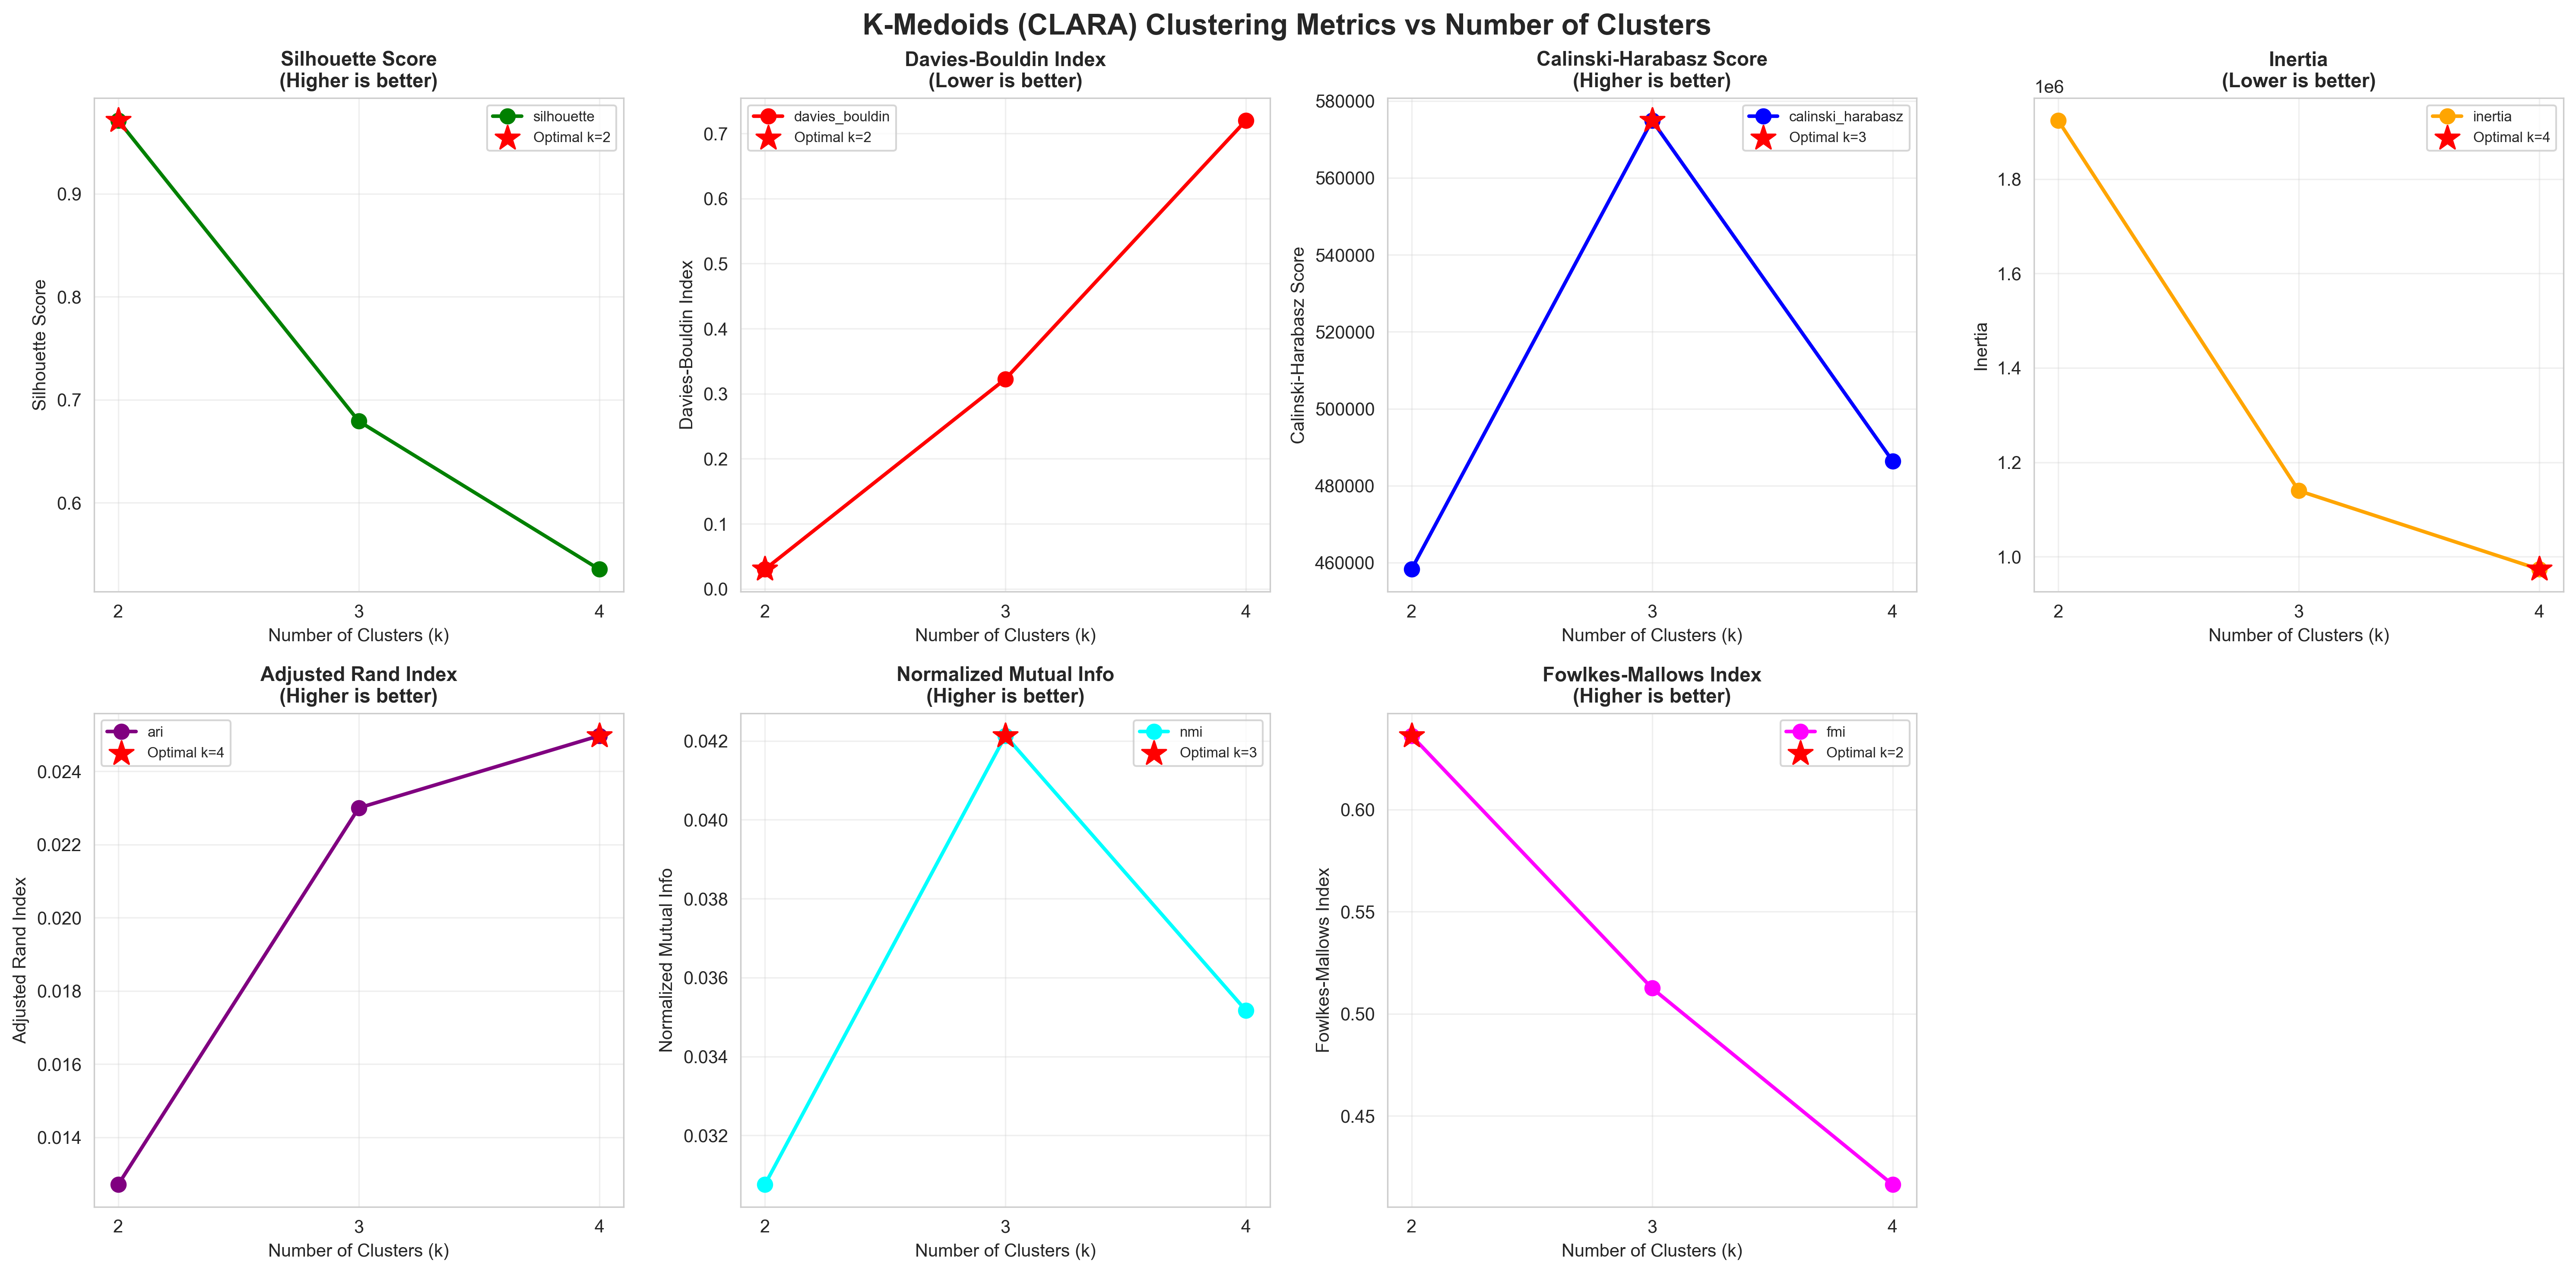
\includegraphics[width=0.95\textwidth]{images/Clarans/predefined/metrics_smote.png}
\caption{Clustering Metrics vs. Number of Clusters for SMOTE Dataset. The optimal value of $k=2$ is marked with red stars across all metrics.}
\label{fig:clara_metrics_smote}
\end{figure}


\subsubsection{Tomek dataset}

\begin{figure}[H]
\centering
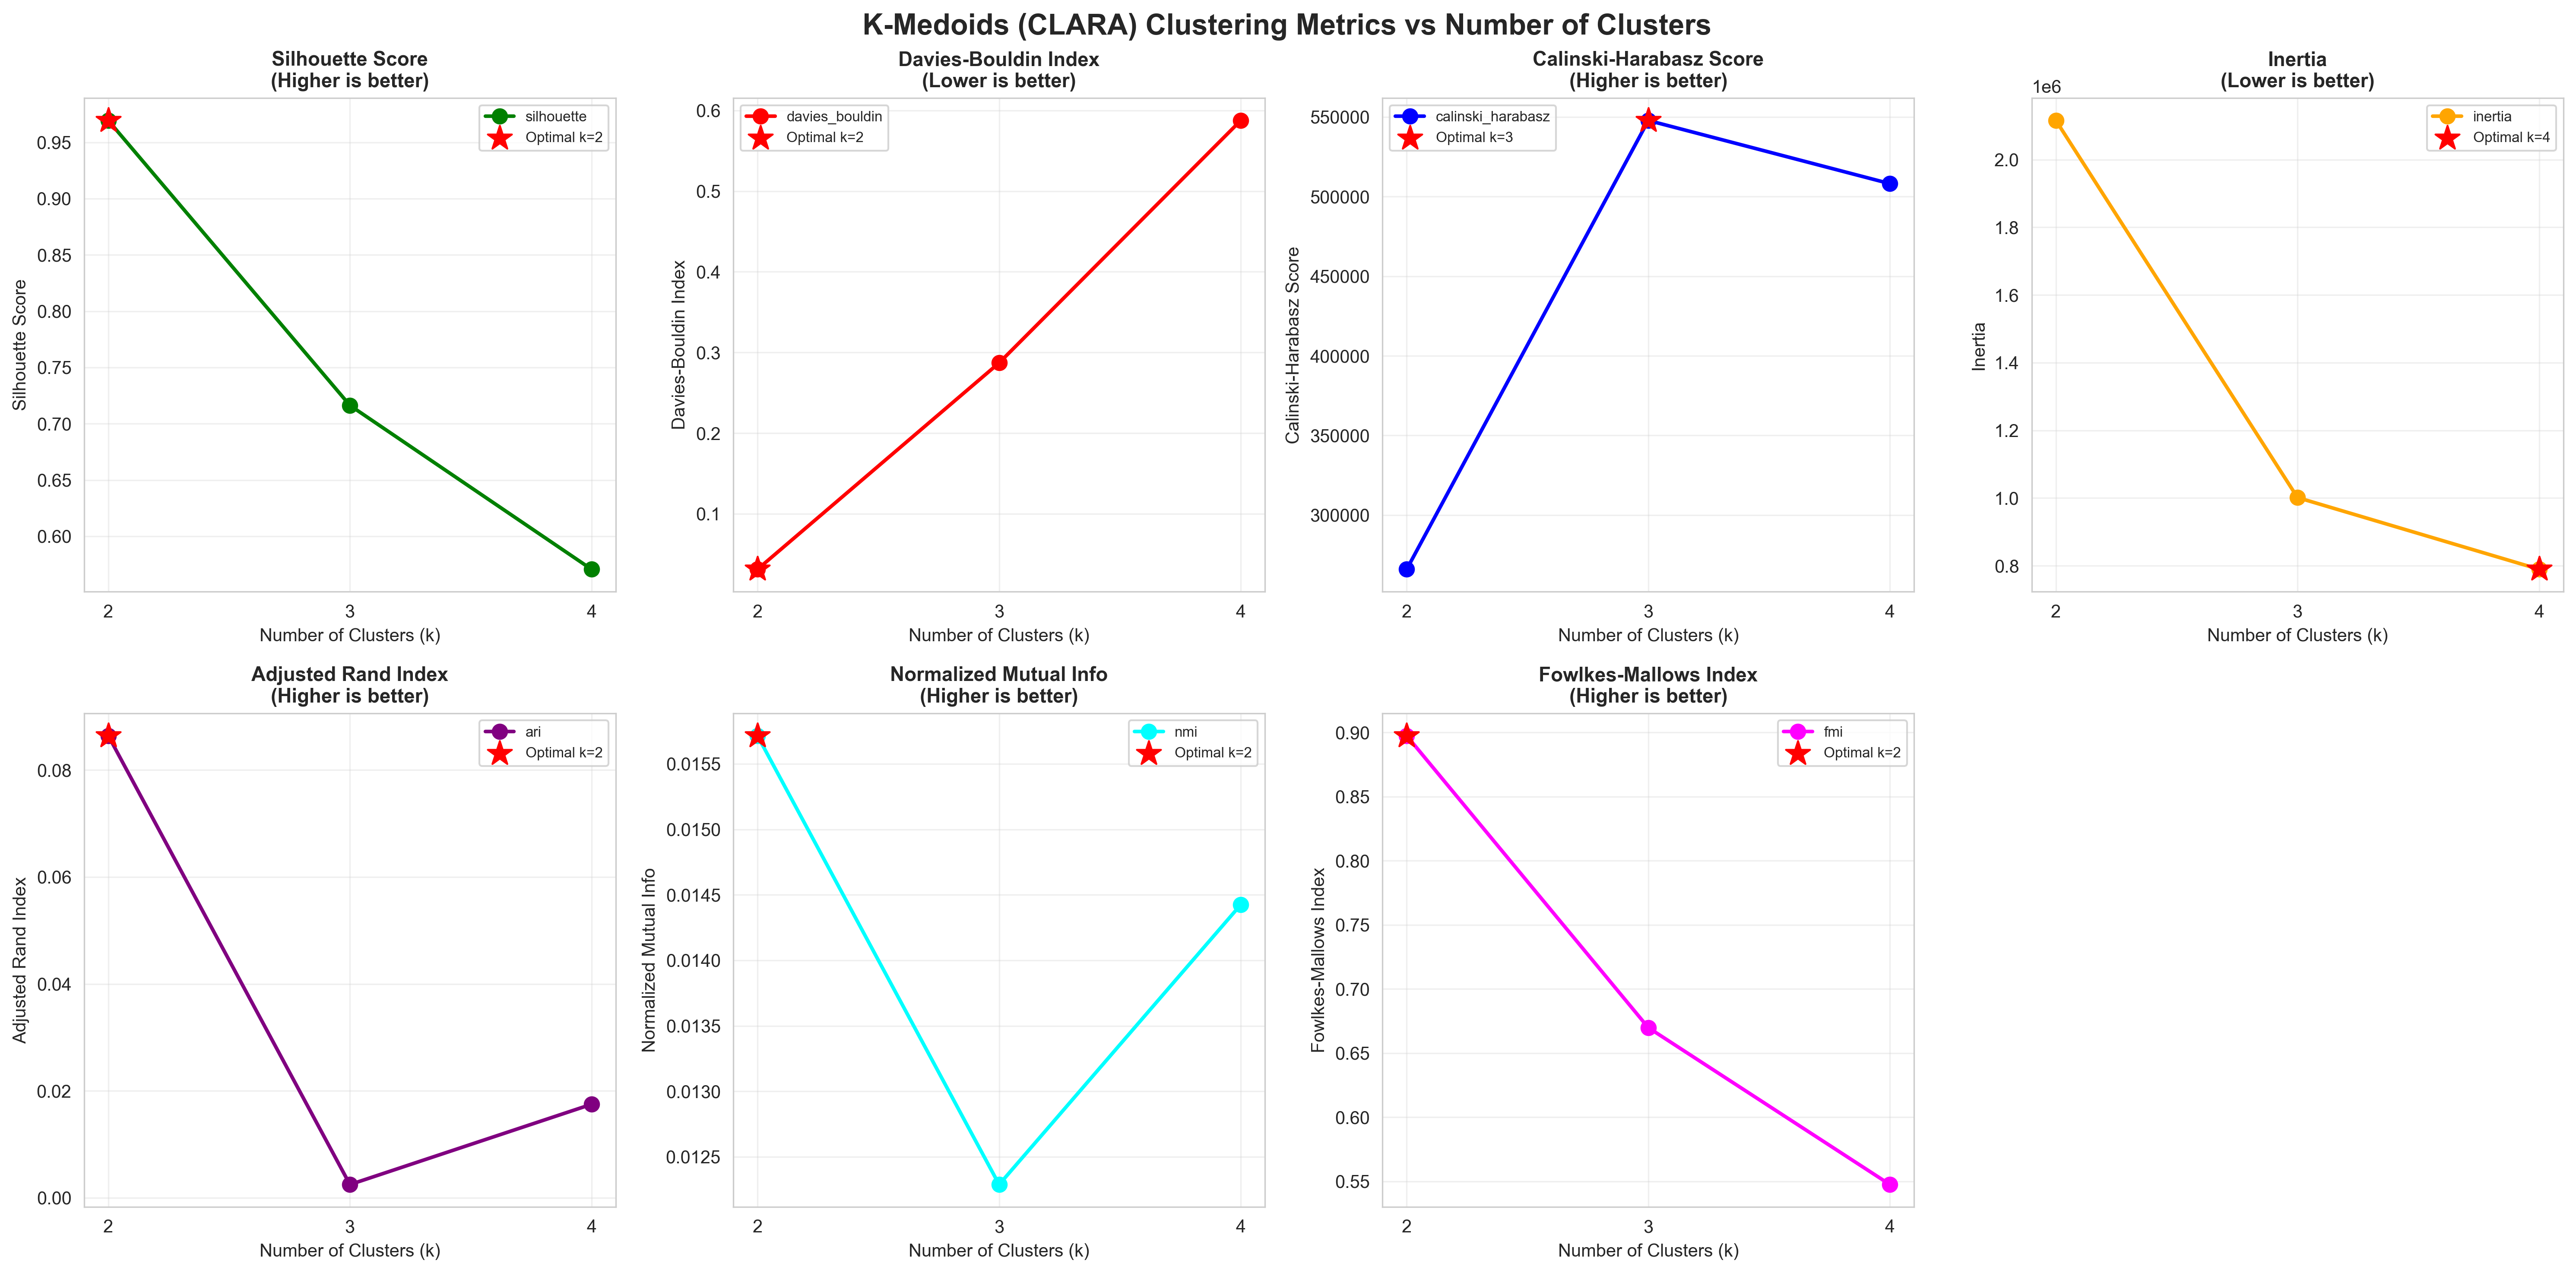
\includegraphics[width=0.95\textwidth]{images/Clarans/predefined/metrics_tomek.png}
\caption{Clustering Metrics vs. Number of Clusters for TOMEK Dataset. The optimal value of $k=2$ is marked with red stars across all metrics.}
% \label{fig:clara_metrics_smote}
\end{figure}

\begin{figure}[H]
\centering
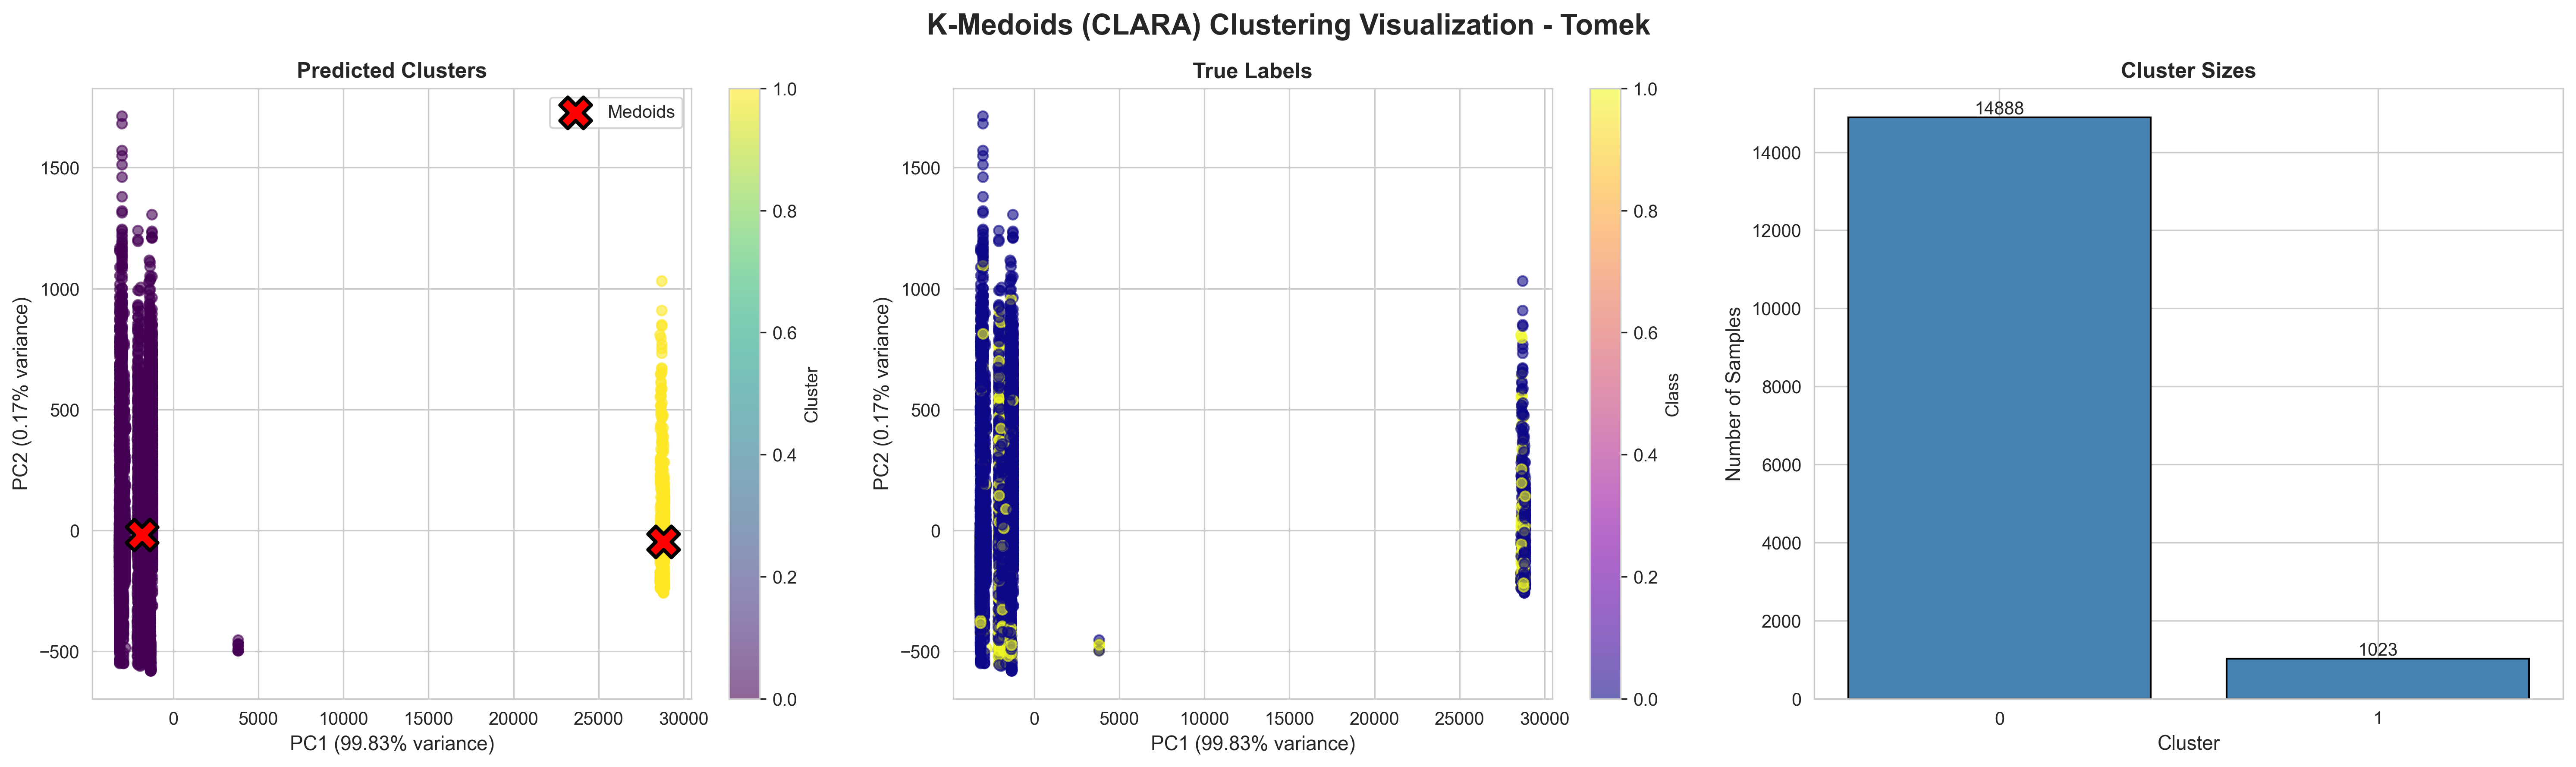
\includegraphics[width=\textwidth]{images/Clarans/predefined/clusters_tomek.png}
\caption{CLARA Clustering Visualization for TOMEK Dataset ($k=2$). Left: Predicted clusters with medoids marked as red crosses. Center: True class labels for comparison. Right: Cluster size distribution showing balanced partitioning.}
% \label{fig:clara_clusters_tomek}
\end{figure}

\subsubsection{Smote-Tomek dataset}

\begin{figure}[H]
\centering
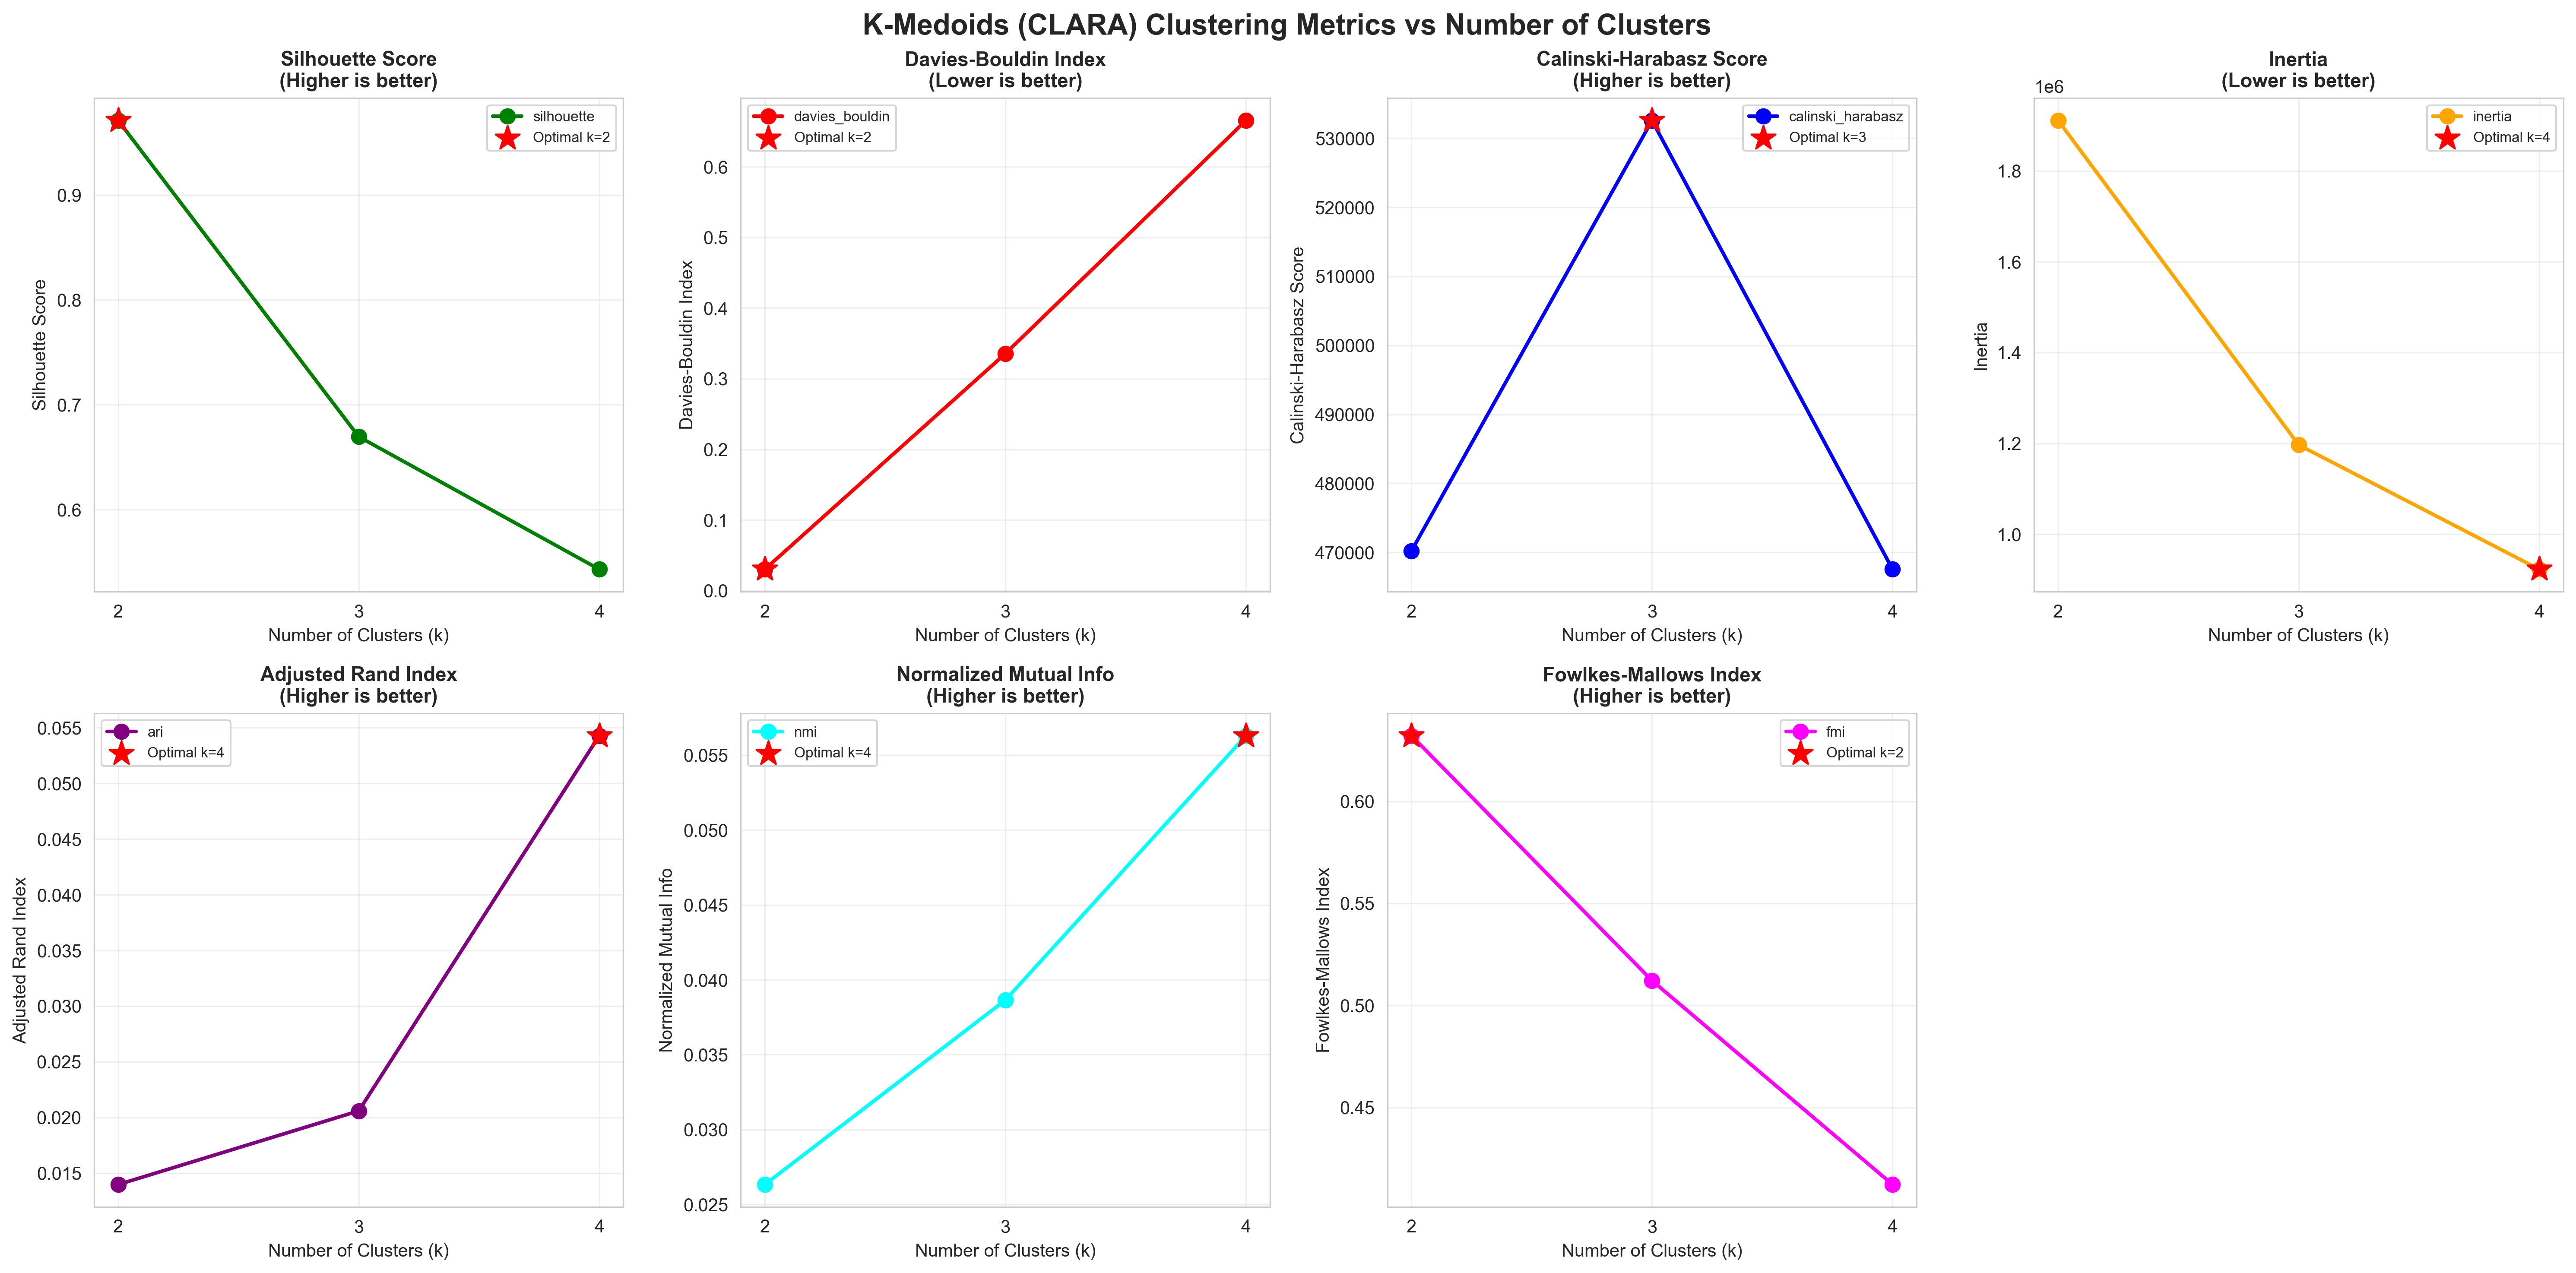
\includegraphics[width=0.95\textwidth]{images/Clarans/predefined/metrics_smote-tomek.png}
\caption{Clustering Metrics vs. Number of Clusters for SMOTE-TOMEK Dataset. The optimal value of $k=2$ is marked with red stars across all metrics.}
% \label{fig:clara_metrics_smote}
\end{figure}

\begin{figure}[H]
\centering
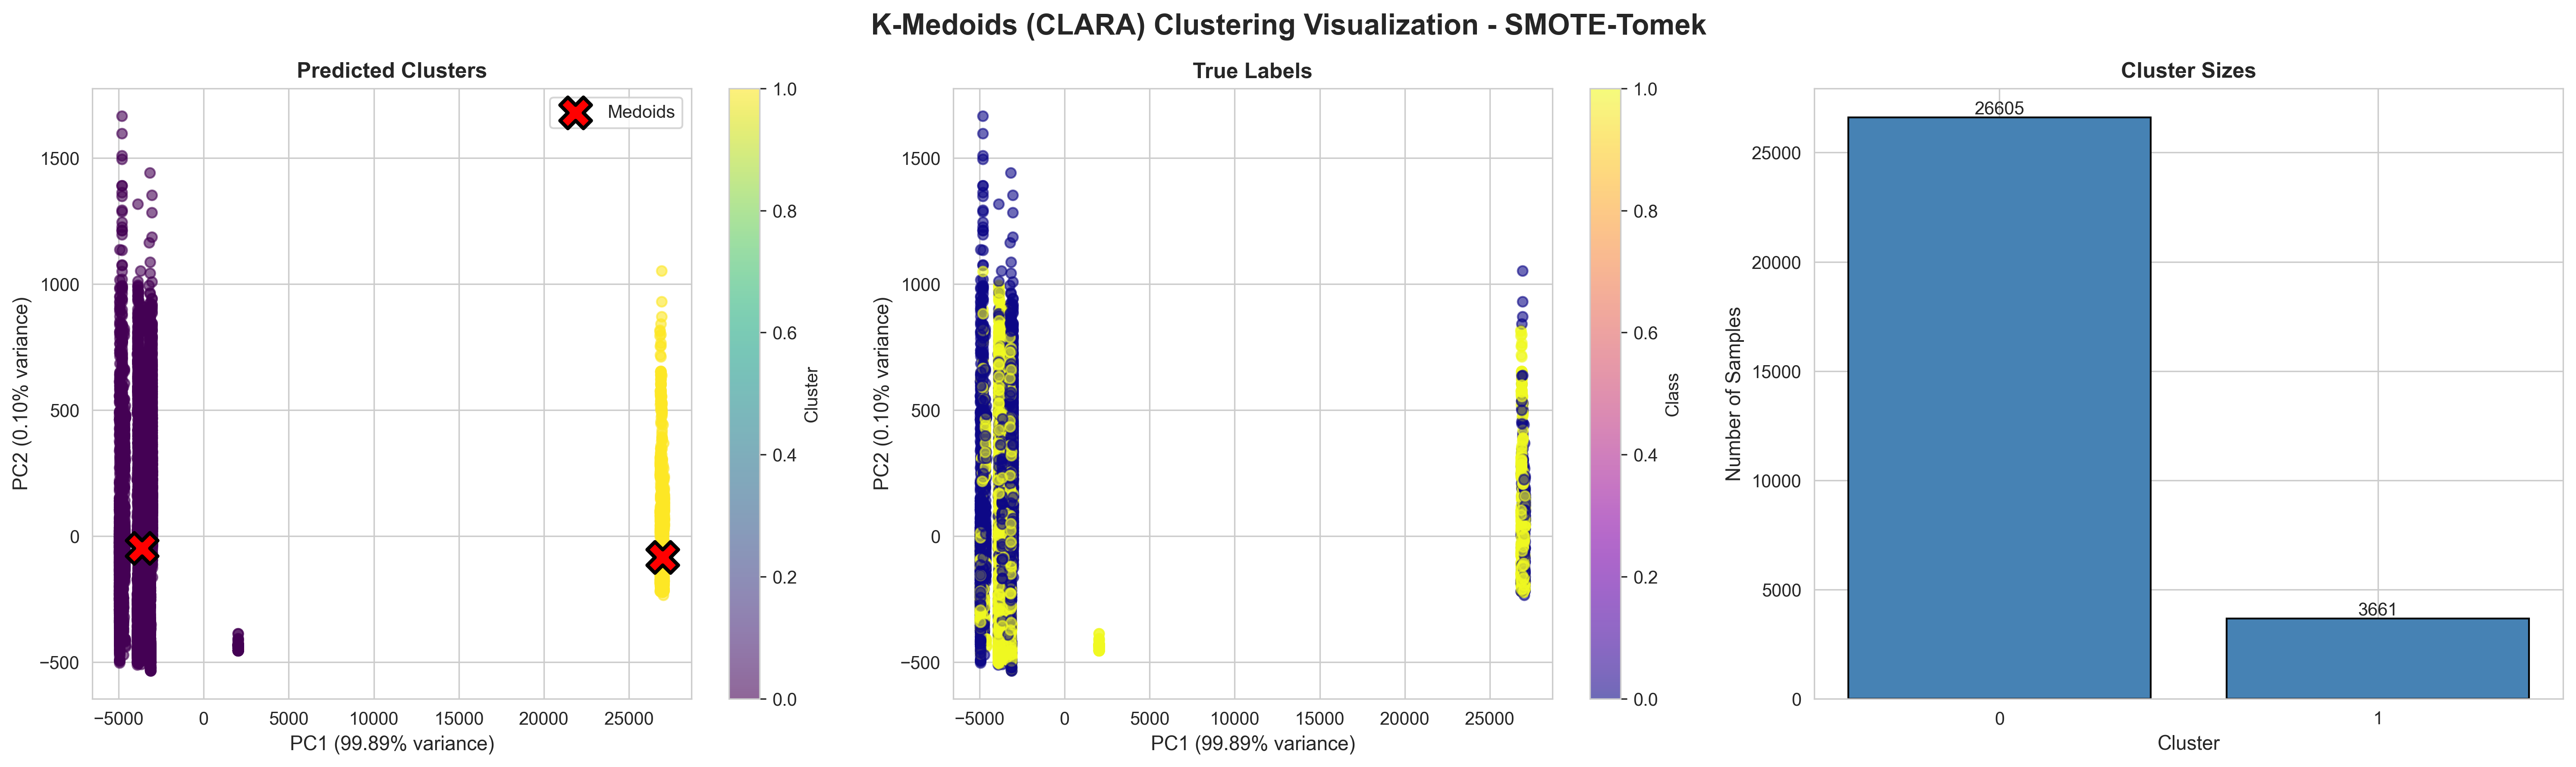
\includegraphics[width=\textwidth]{images/Clarans/predefined/clusters_smote-tomek.png}
\caption{CLARA Clustering Visualization for SMOTE-TOMEK Dataset ($k=2$). Left: Predicted clusters with medoids marked as red crosses. Center: True class labels for comparison. Right: Cluster size distribution showing balanced partitioning.}
% \label{fig:clara_clusters_smote}
\end{figure}


\subsubsection{Cross-Dataset Comparison}

\begin{figure}[H]
\centering
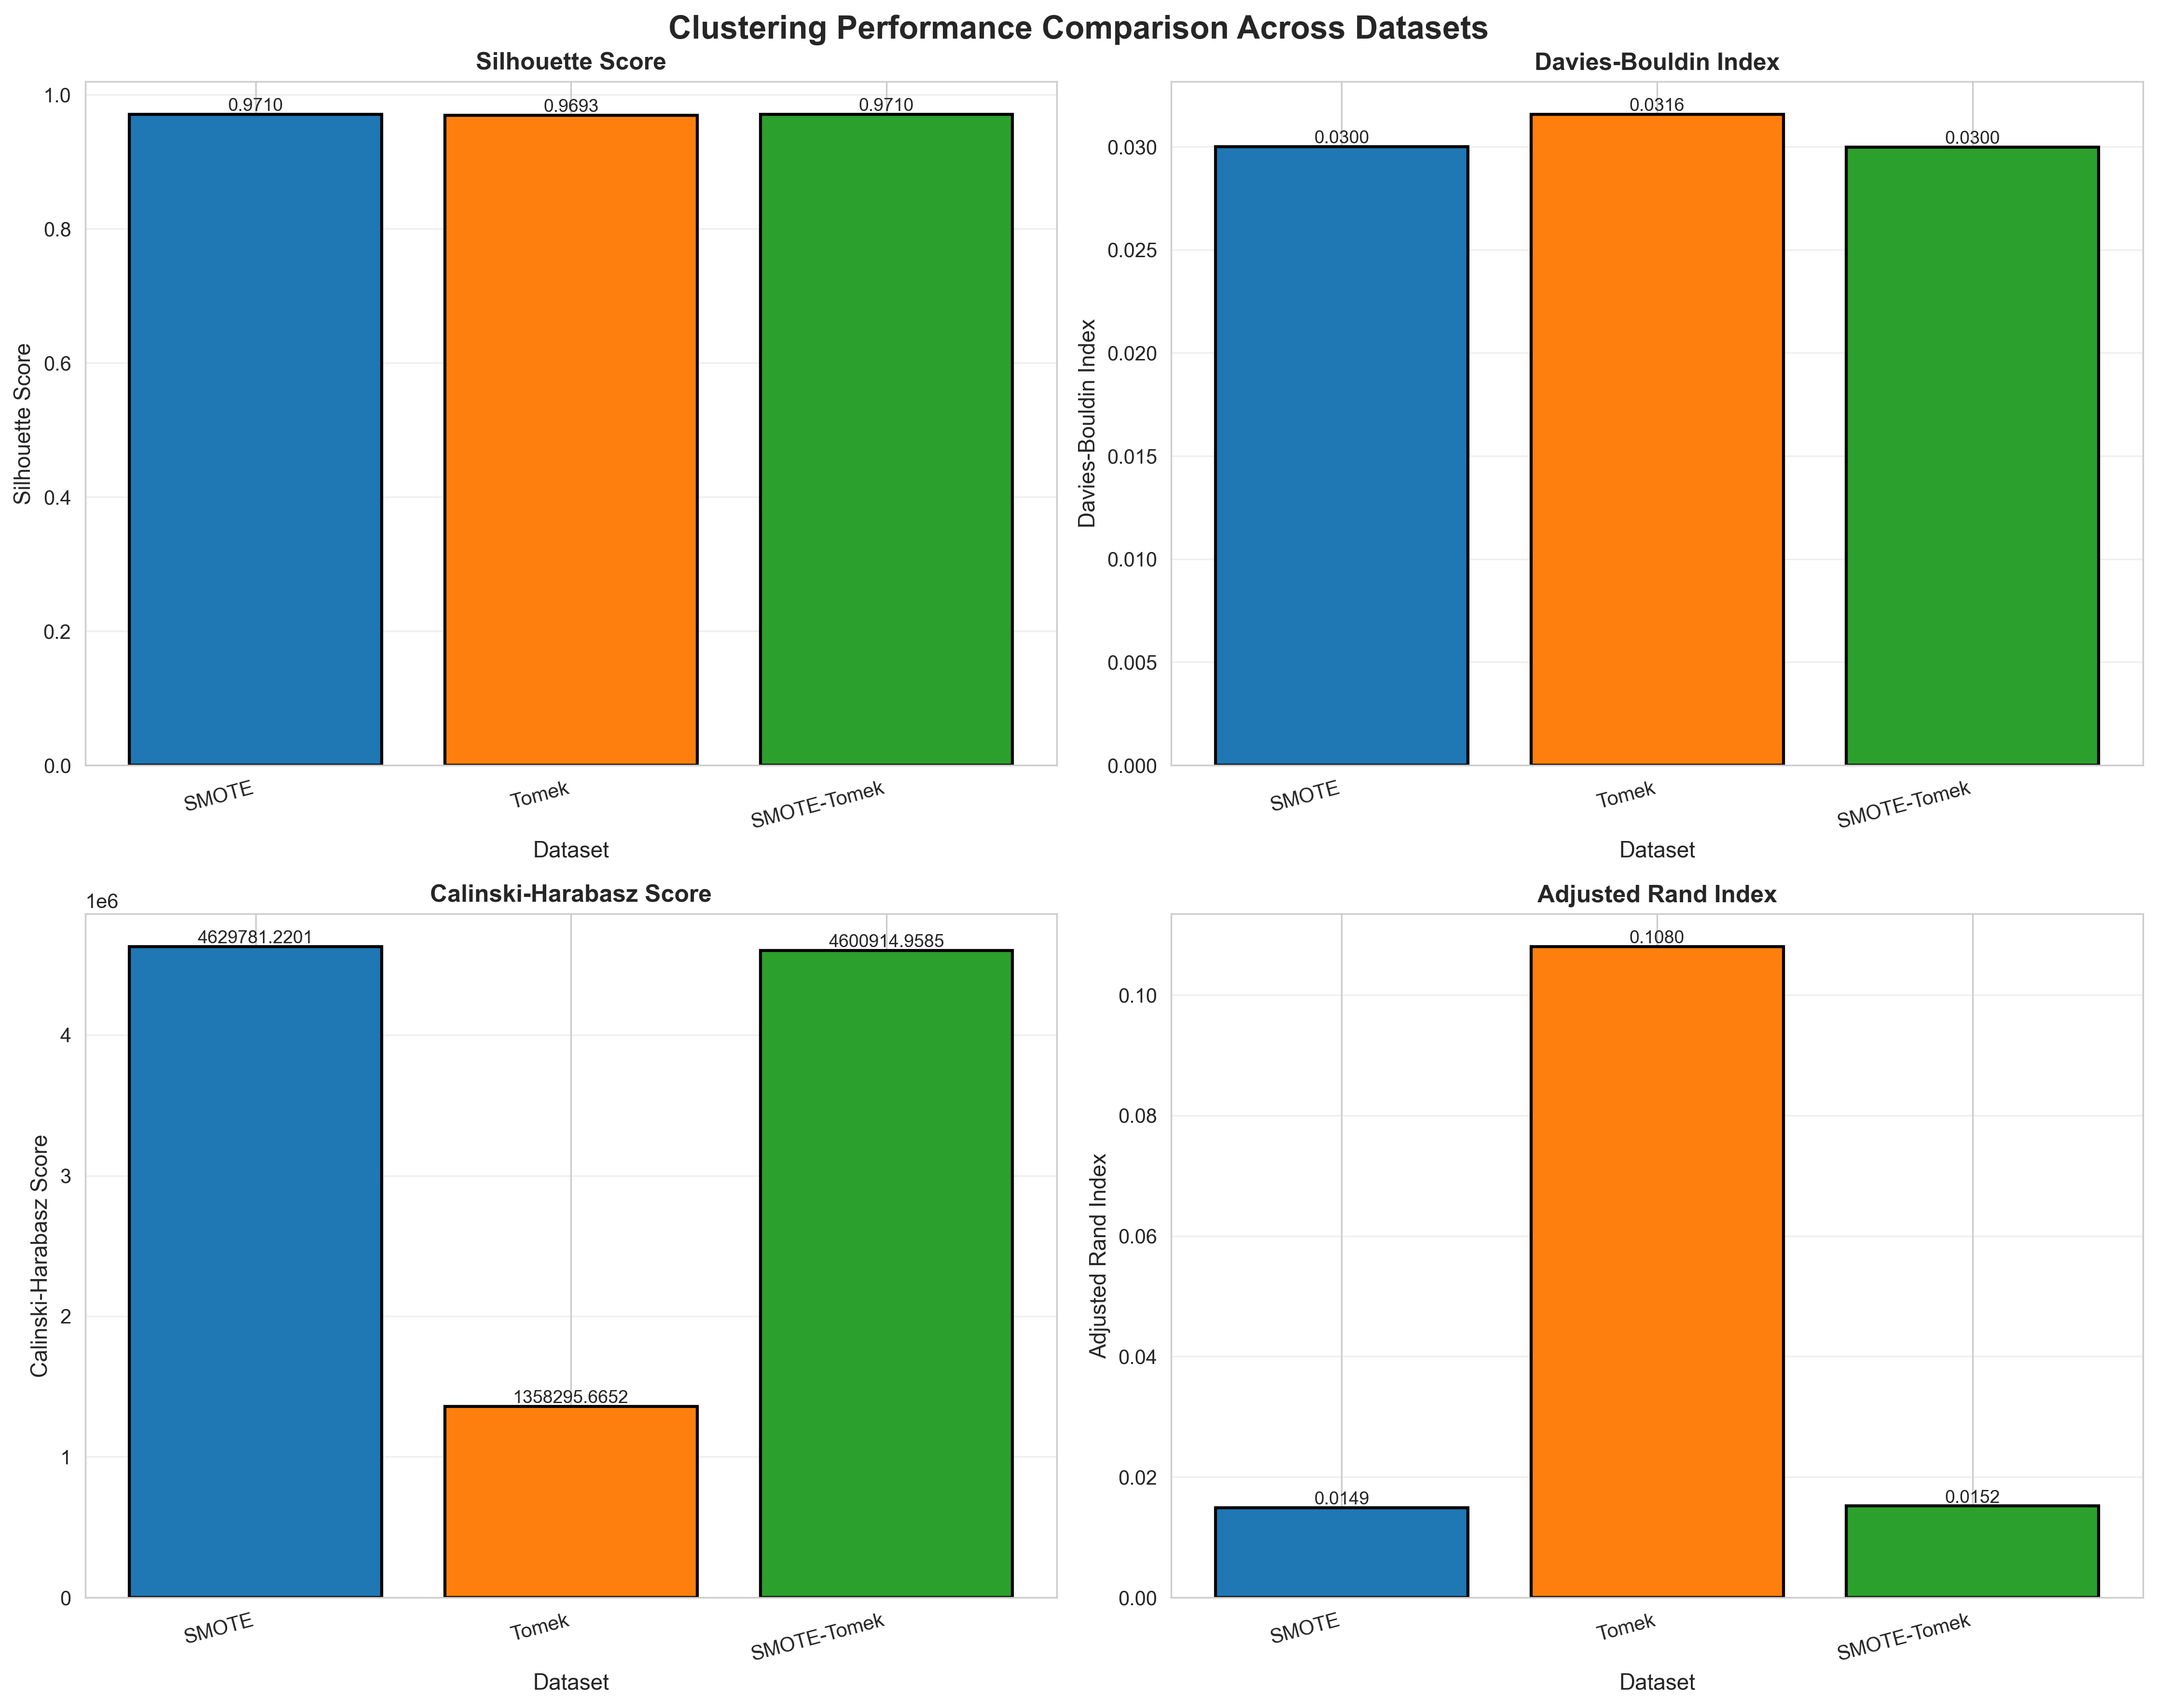
\includegraphics[width=0.6\textwidth]{images/Clarans/predefined/clustering_comparison.png}
\caption{Performance Comparison of CLARA Across Resampling Methods. All datasets achieved similar Silhouette Scores (>0.96), while Tomek showed superior alignment with true labels (highest ARI and Fowlkes-Mallows Score).}
\label{fig:clara_comparison}
\end{figure}

The comparison across resampling methods reveals consistent clustering quality, with all datasets achieving Silhouette Scores exceeding 0.96 and Davies-Bouldin indices below 0.032. The Tomek dataset's superior ARI (0.1080) and Fowlkes-Mallows Score (0.8967) suggest that removing noisy boundary samples enhances the results. The SMOTE and SMOTE-Tomek datasets, while producing equally compact clusters, show lower external validation metrics, indicating that synthetic sample generation introduces variability that creates natural groupings different from the original class structure.



\subsection{Bayesian Optimization}


\begin{figure}[H]
\centering
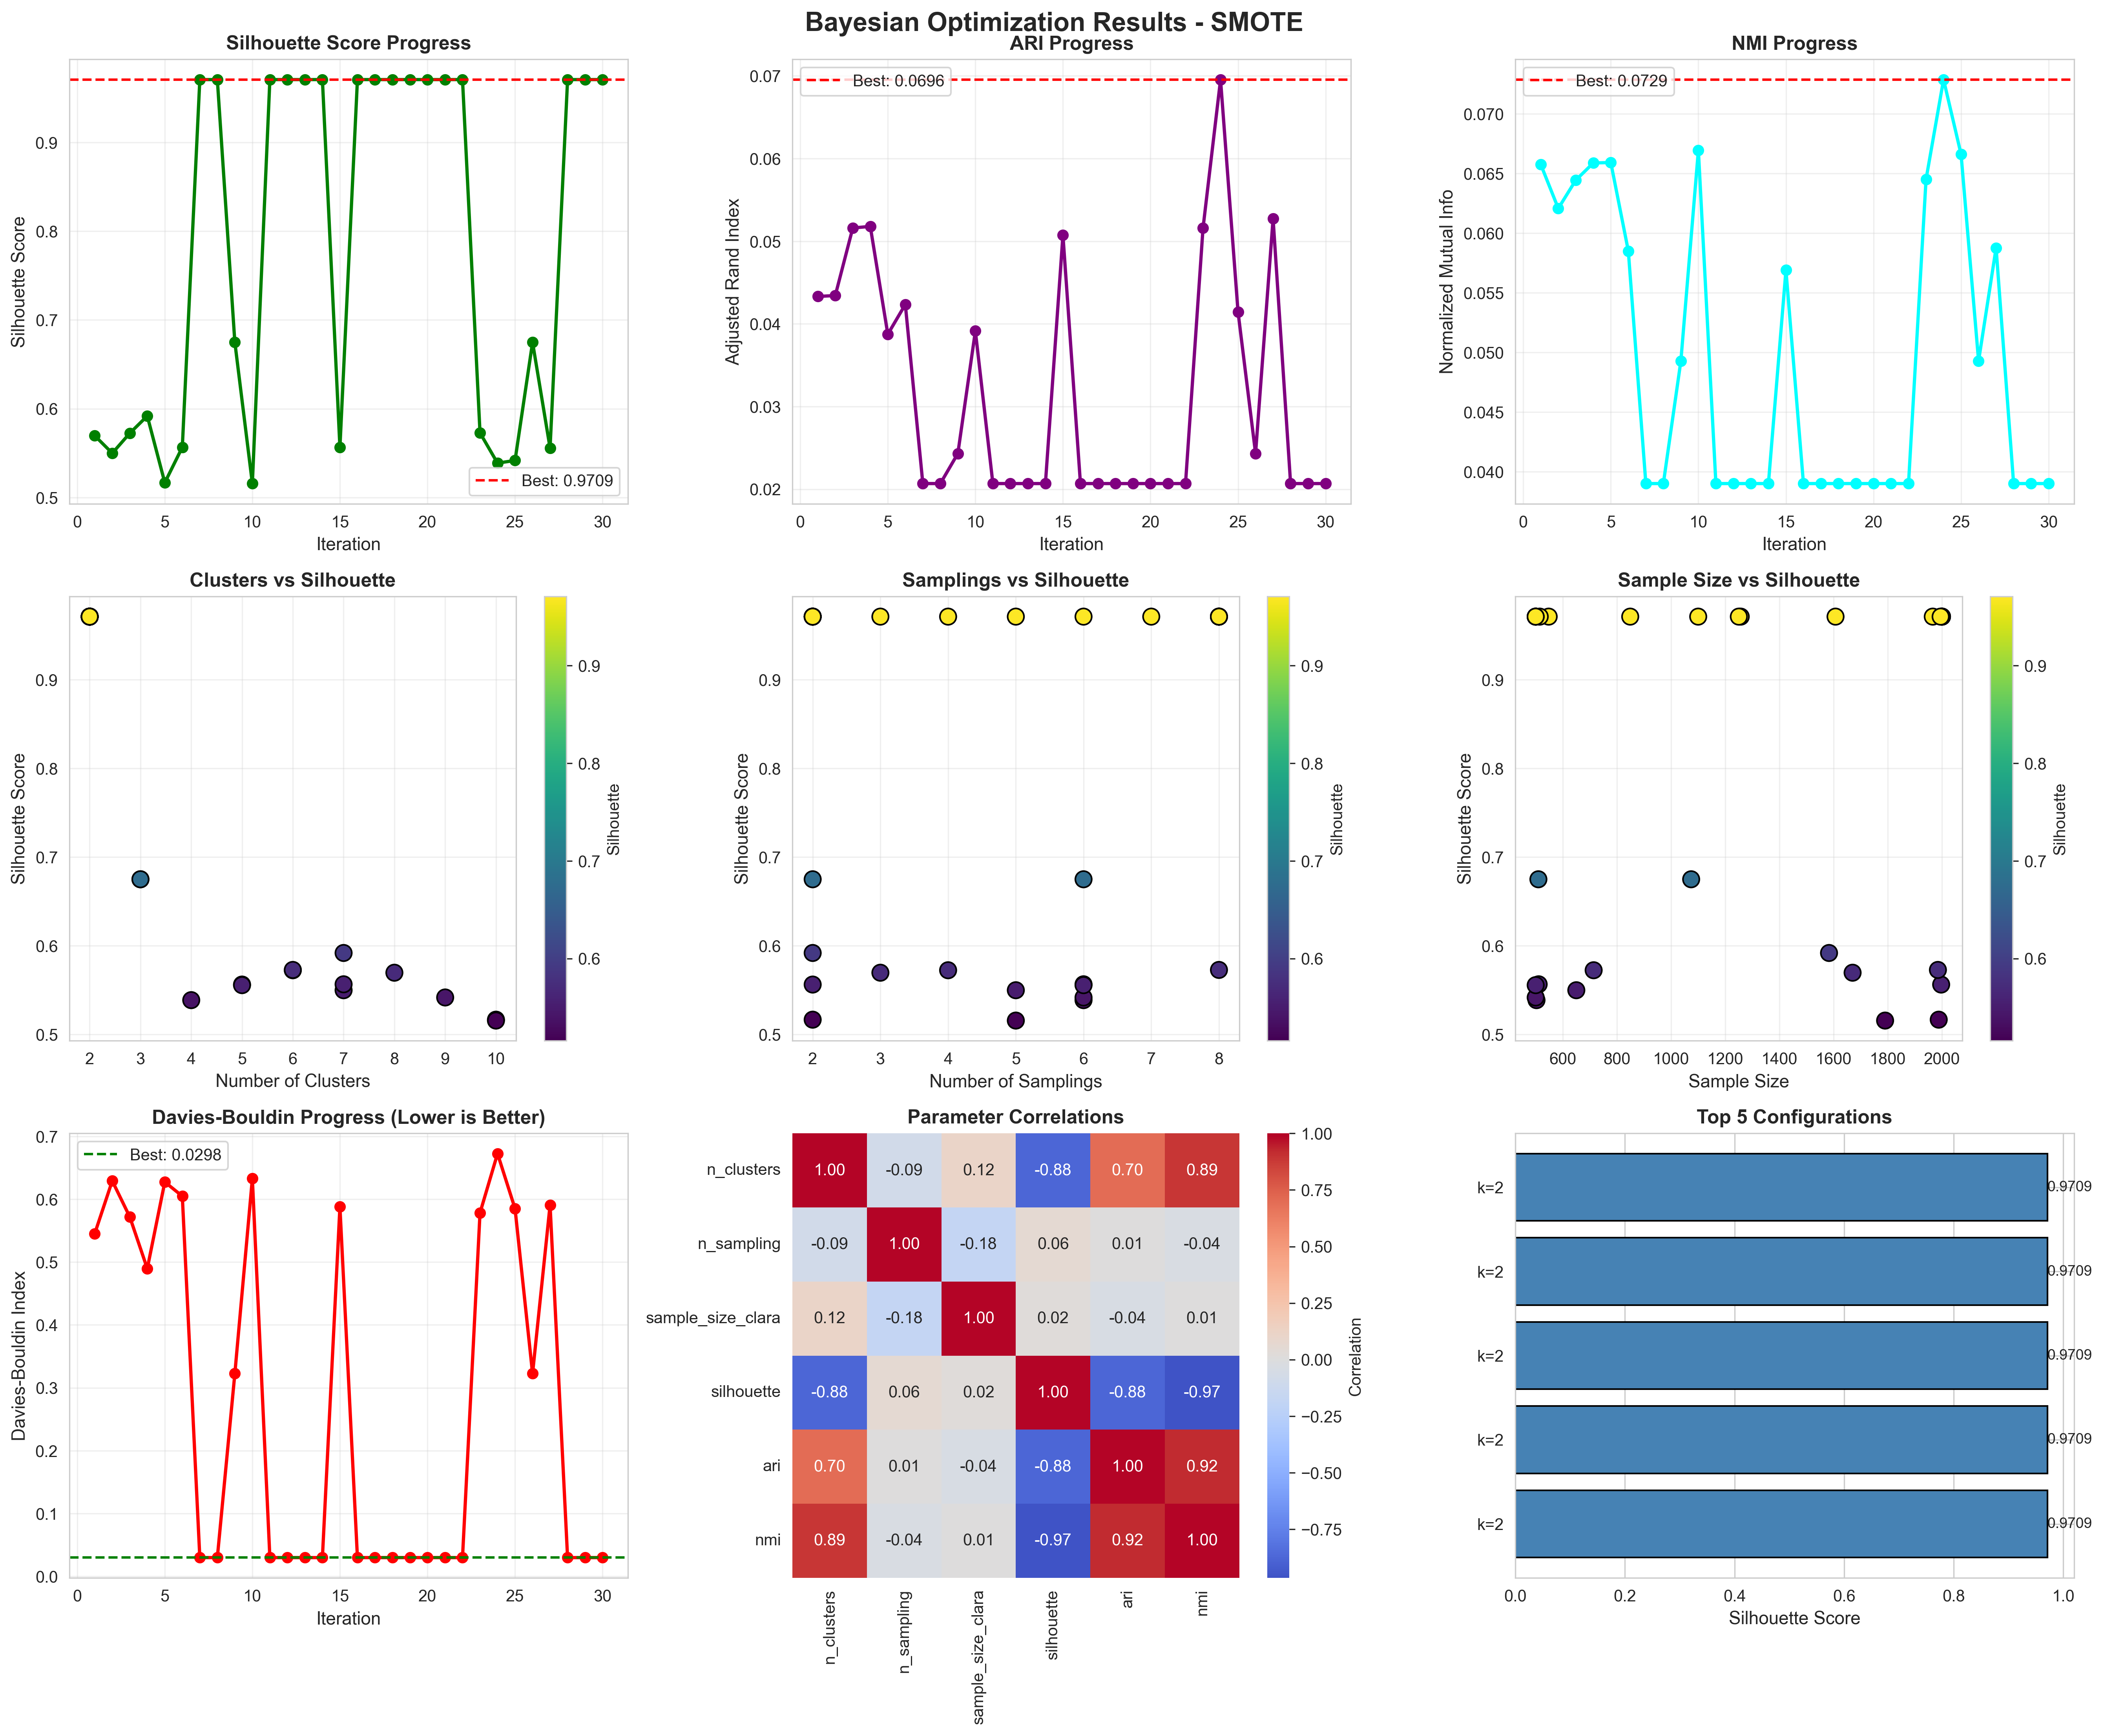
\includegraphics[width=0.9\textwidth]{images/Clarans/bayesopt/bayesian_optimization_smote.png}
\caption{Bayesian Optimization Progress for SMOTE Dataset. Top row: Evolution of clustering metrics across 30 iterations. Bottom row: Parameter impact on Silhouette Score, parameter correlation heatmap, and top 5 configurations. The algorithm rapidly converged to $k=2$ after exploring higher values of $k$ in early iterations.}
\label{fig:clara_bayesian}
\end{figure}

The optimization trace reveals that the algorithm quickly identified the superior performance of $k=2$ (Silhouette Score ~0.97) compared to larger cluster counts ($k \geq 3$: Silhouette ~0.54-0.67). After the initial exploration phase (iterations 1-6), Bayesian Optimization predominantly sampled $k=2$ configurations, demonstrating efficient convergence. The parameter correlation heatmap shows weak correlations between hyperparameters, indicating that the number of clusters dominates performance, while sampling parameters have minimal impact within reasonable ranges.



\subsubsection{Tomek dataset}
\begin{figure}[H]
\centering
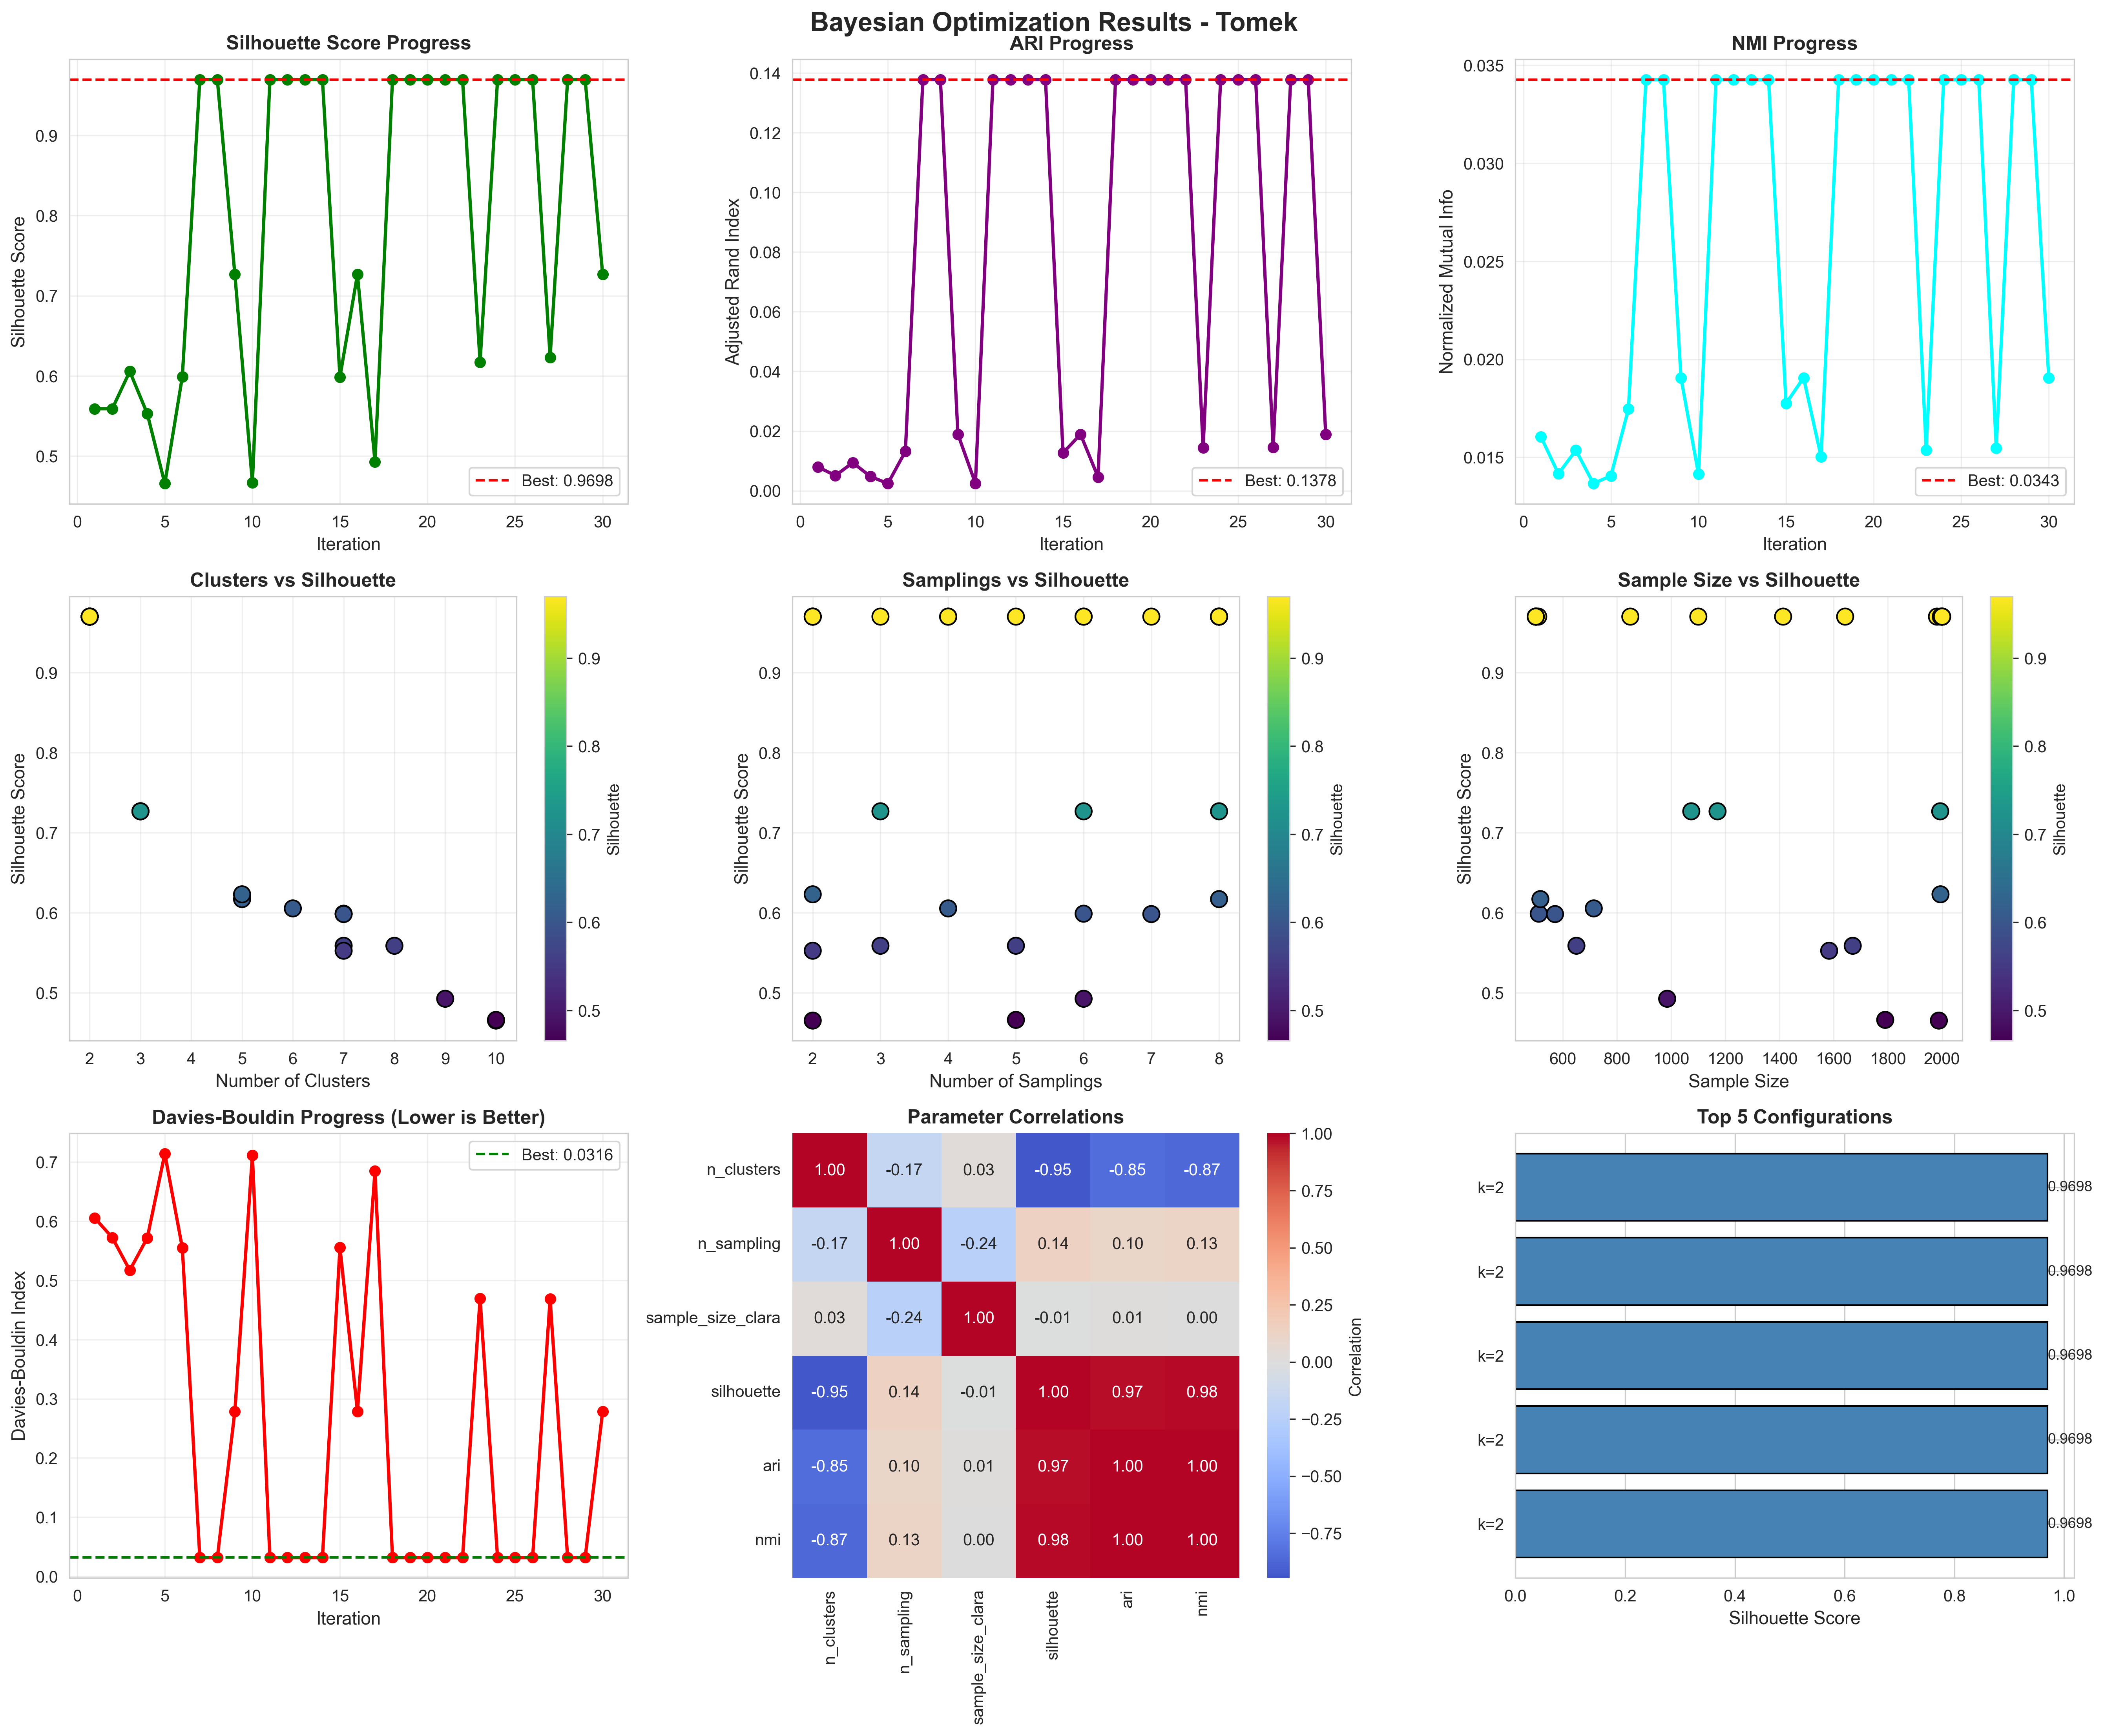
\includegraphics[width=0.9\textwidth]{images/Clarans/bayesopt/bayesian_optimization_tomek.png}
\caption{Bayesian Optimization Progress for TOMEK Dataset. Top row: Evolution of clustering metrics across 30 iterations. Bottom row: Parameter impact on Silhouette Score, parameter correlation heatmap, and top 5 configurations. The algorithm rapidly converged to $k=2$ after exploring higher values of $k$ in early iterations.}
\end{figure}

\subsubsection{Smote-Tomek dataset}
\begin{figure}[H]
\centering
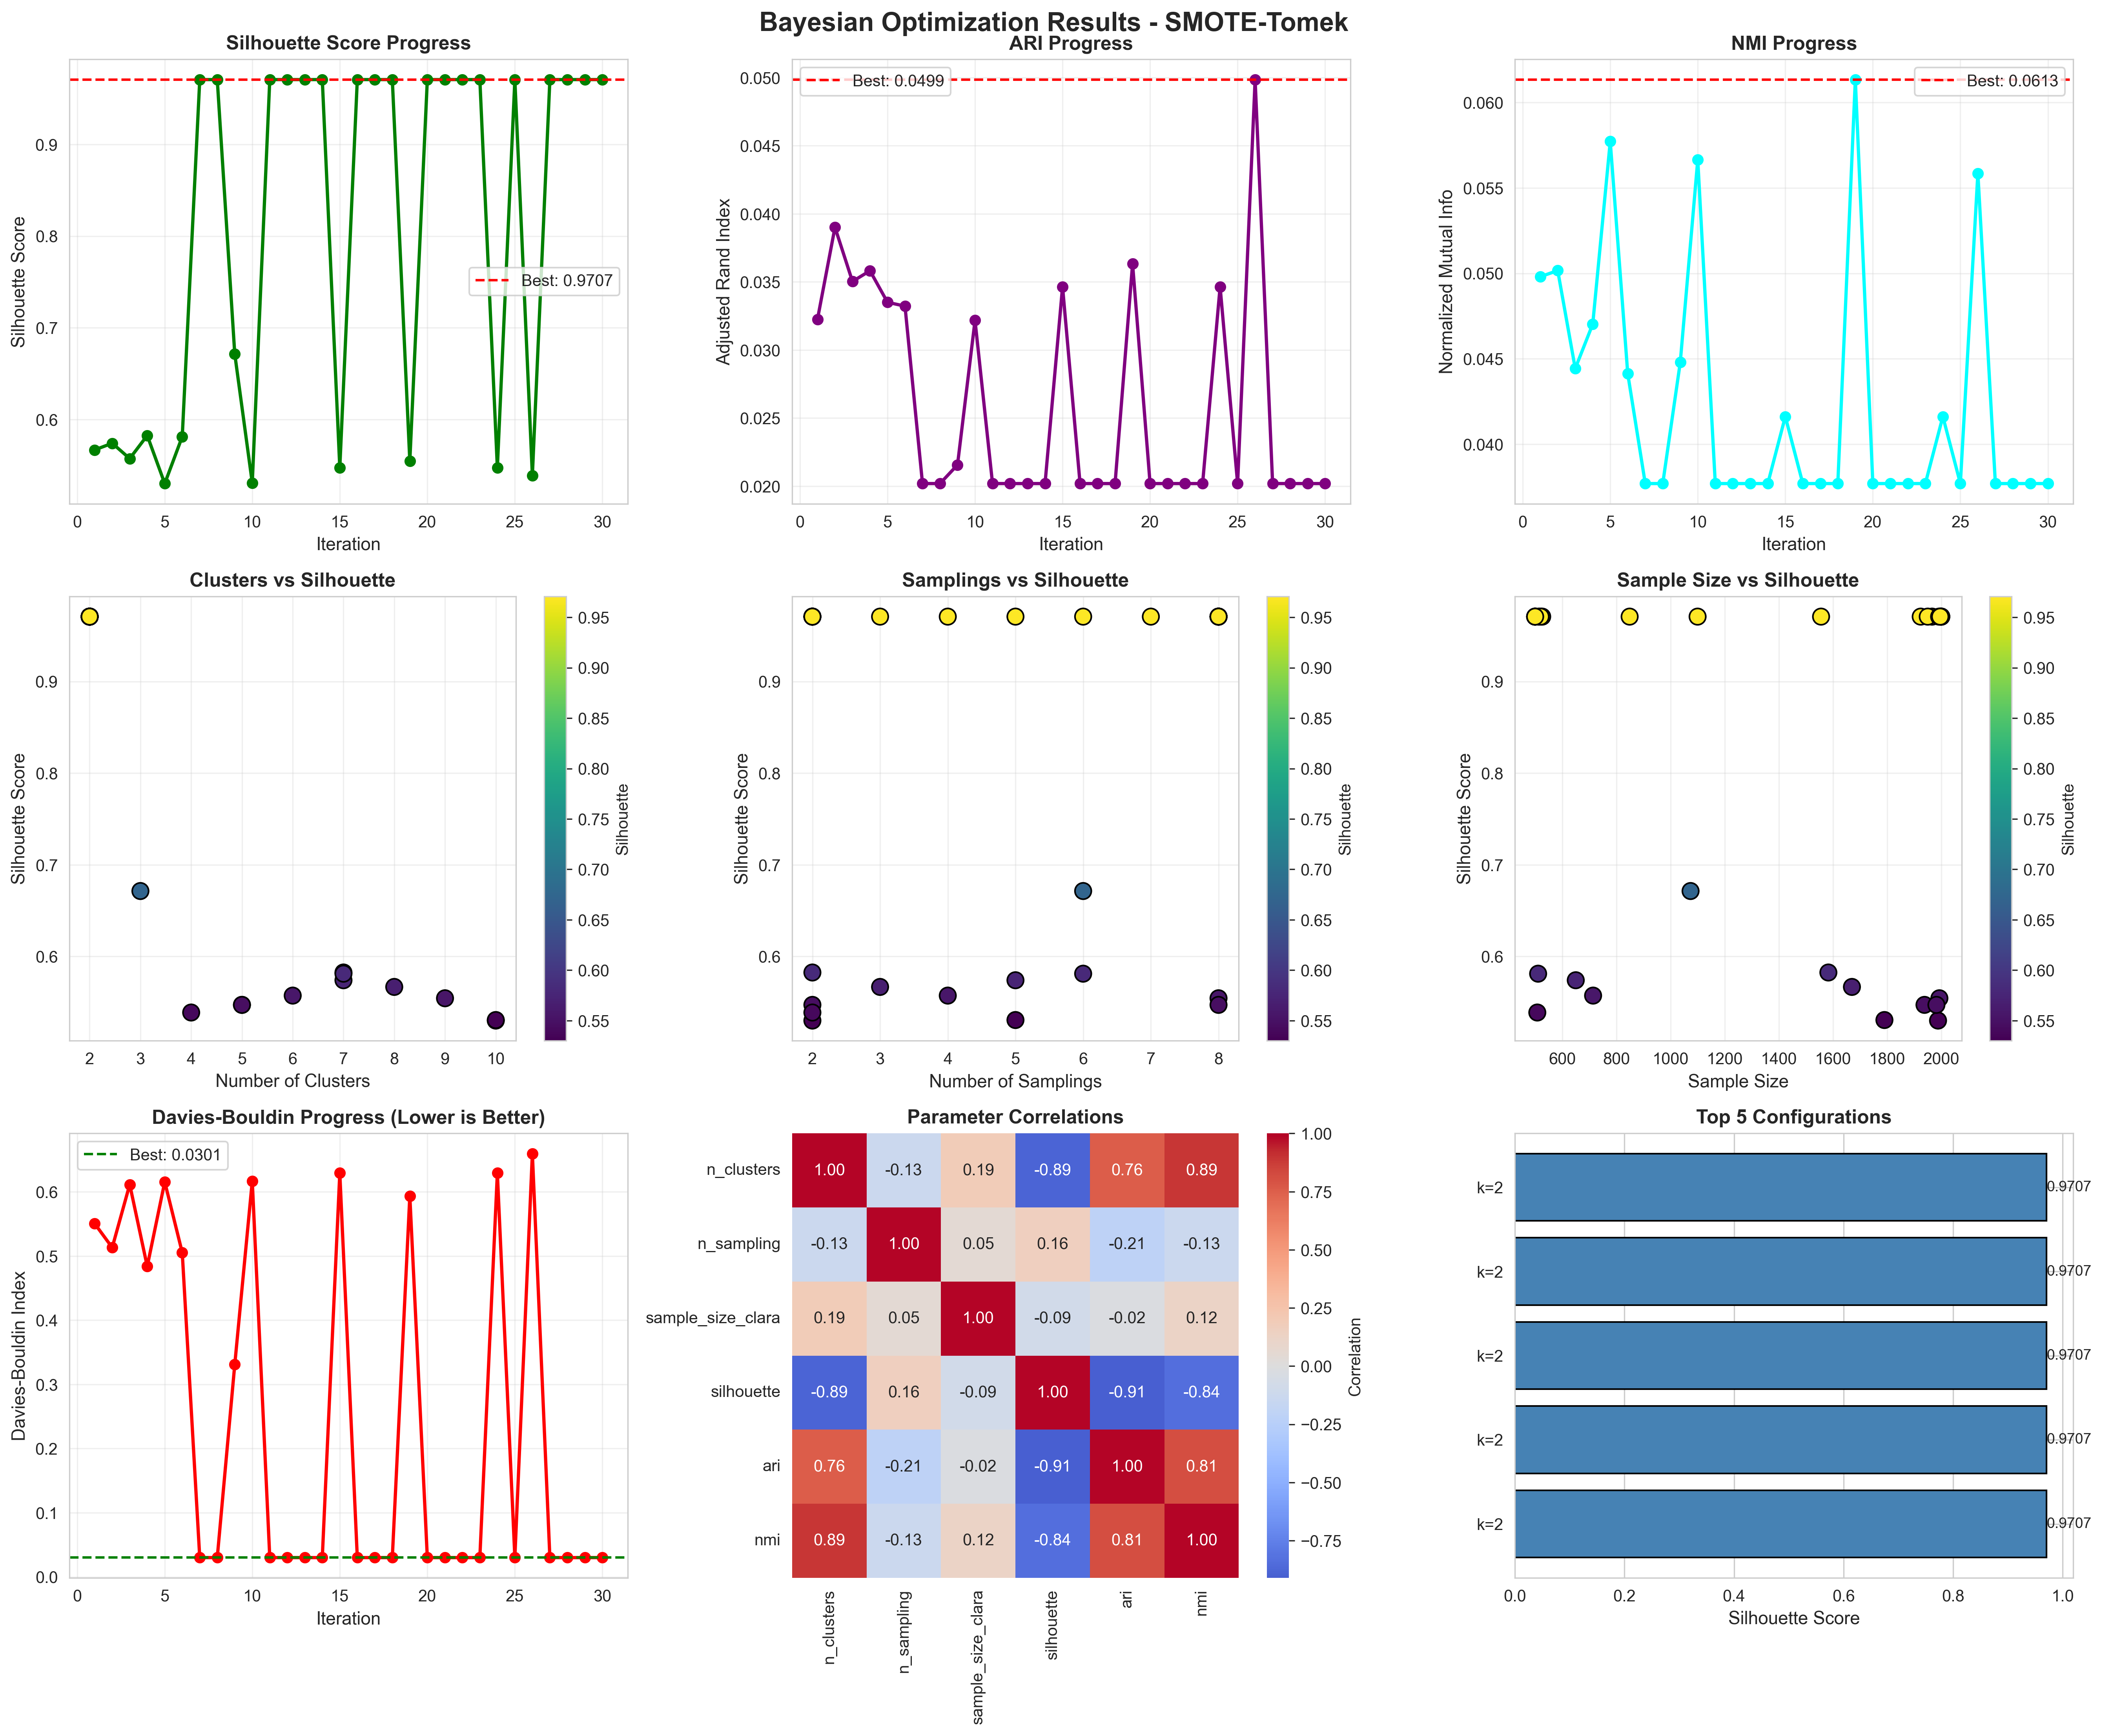
\includegraphics[width=0.9\textwidth]{images/Clarans/bayesopt/bayesian_optimization_smote-tomek.png}
\caption{Bayesian Optimization Progress for SMOTE-TOMEK Dataset. Top row: Evolution of clustering metrics across 30 iterations. Bottom row: Parameter impact on Silhouette Score, parameter correlation heatmap, and top 5 configurations. The algorithm rapidly converged to $k=2$ after exploring higher values of $k$ in early iterations.}
\end{figure}

\subsubsection{Comparison of all datasets}
\begin{figure}[H]
\centering
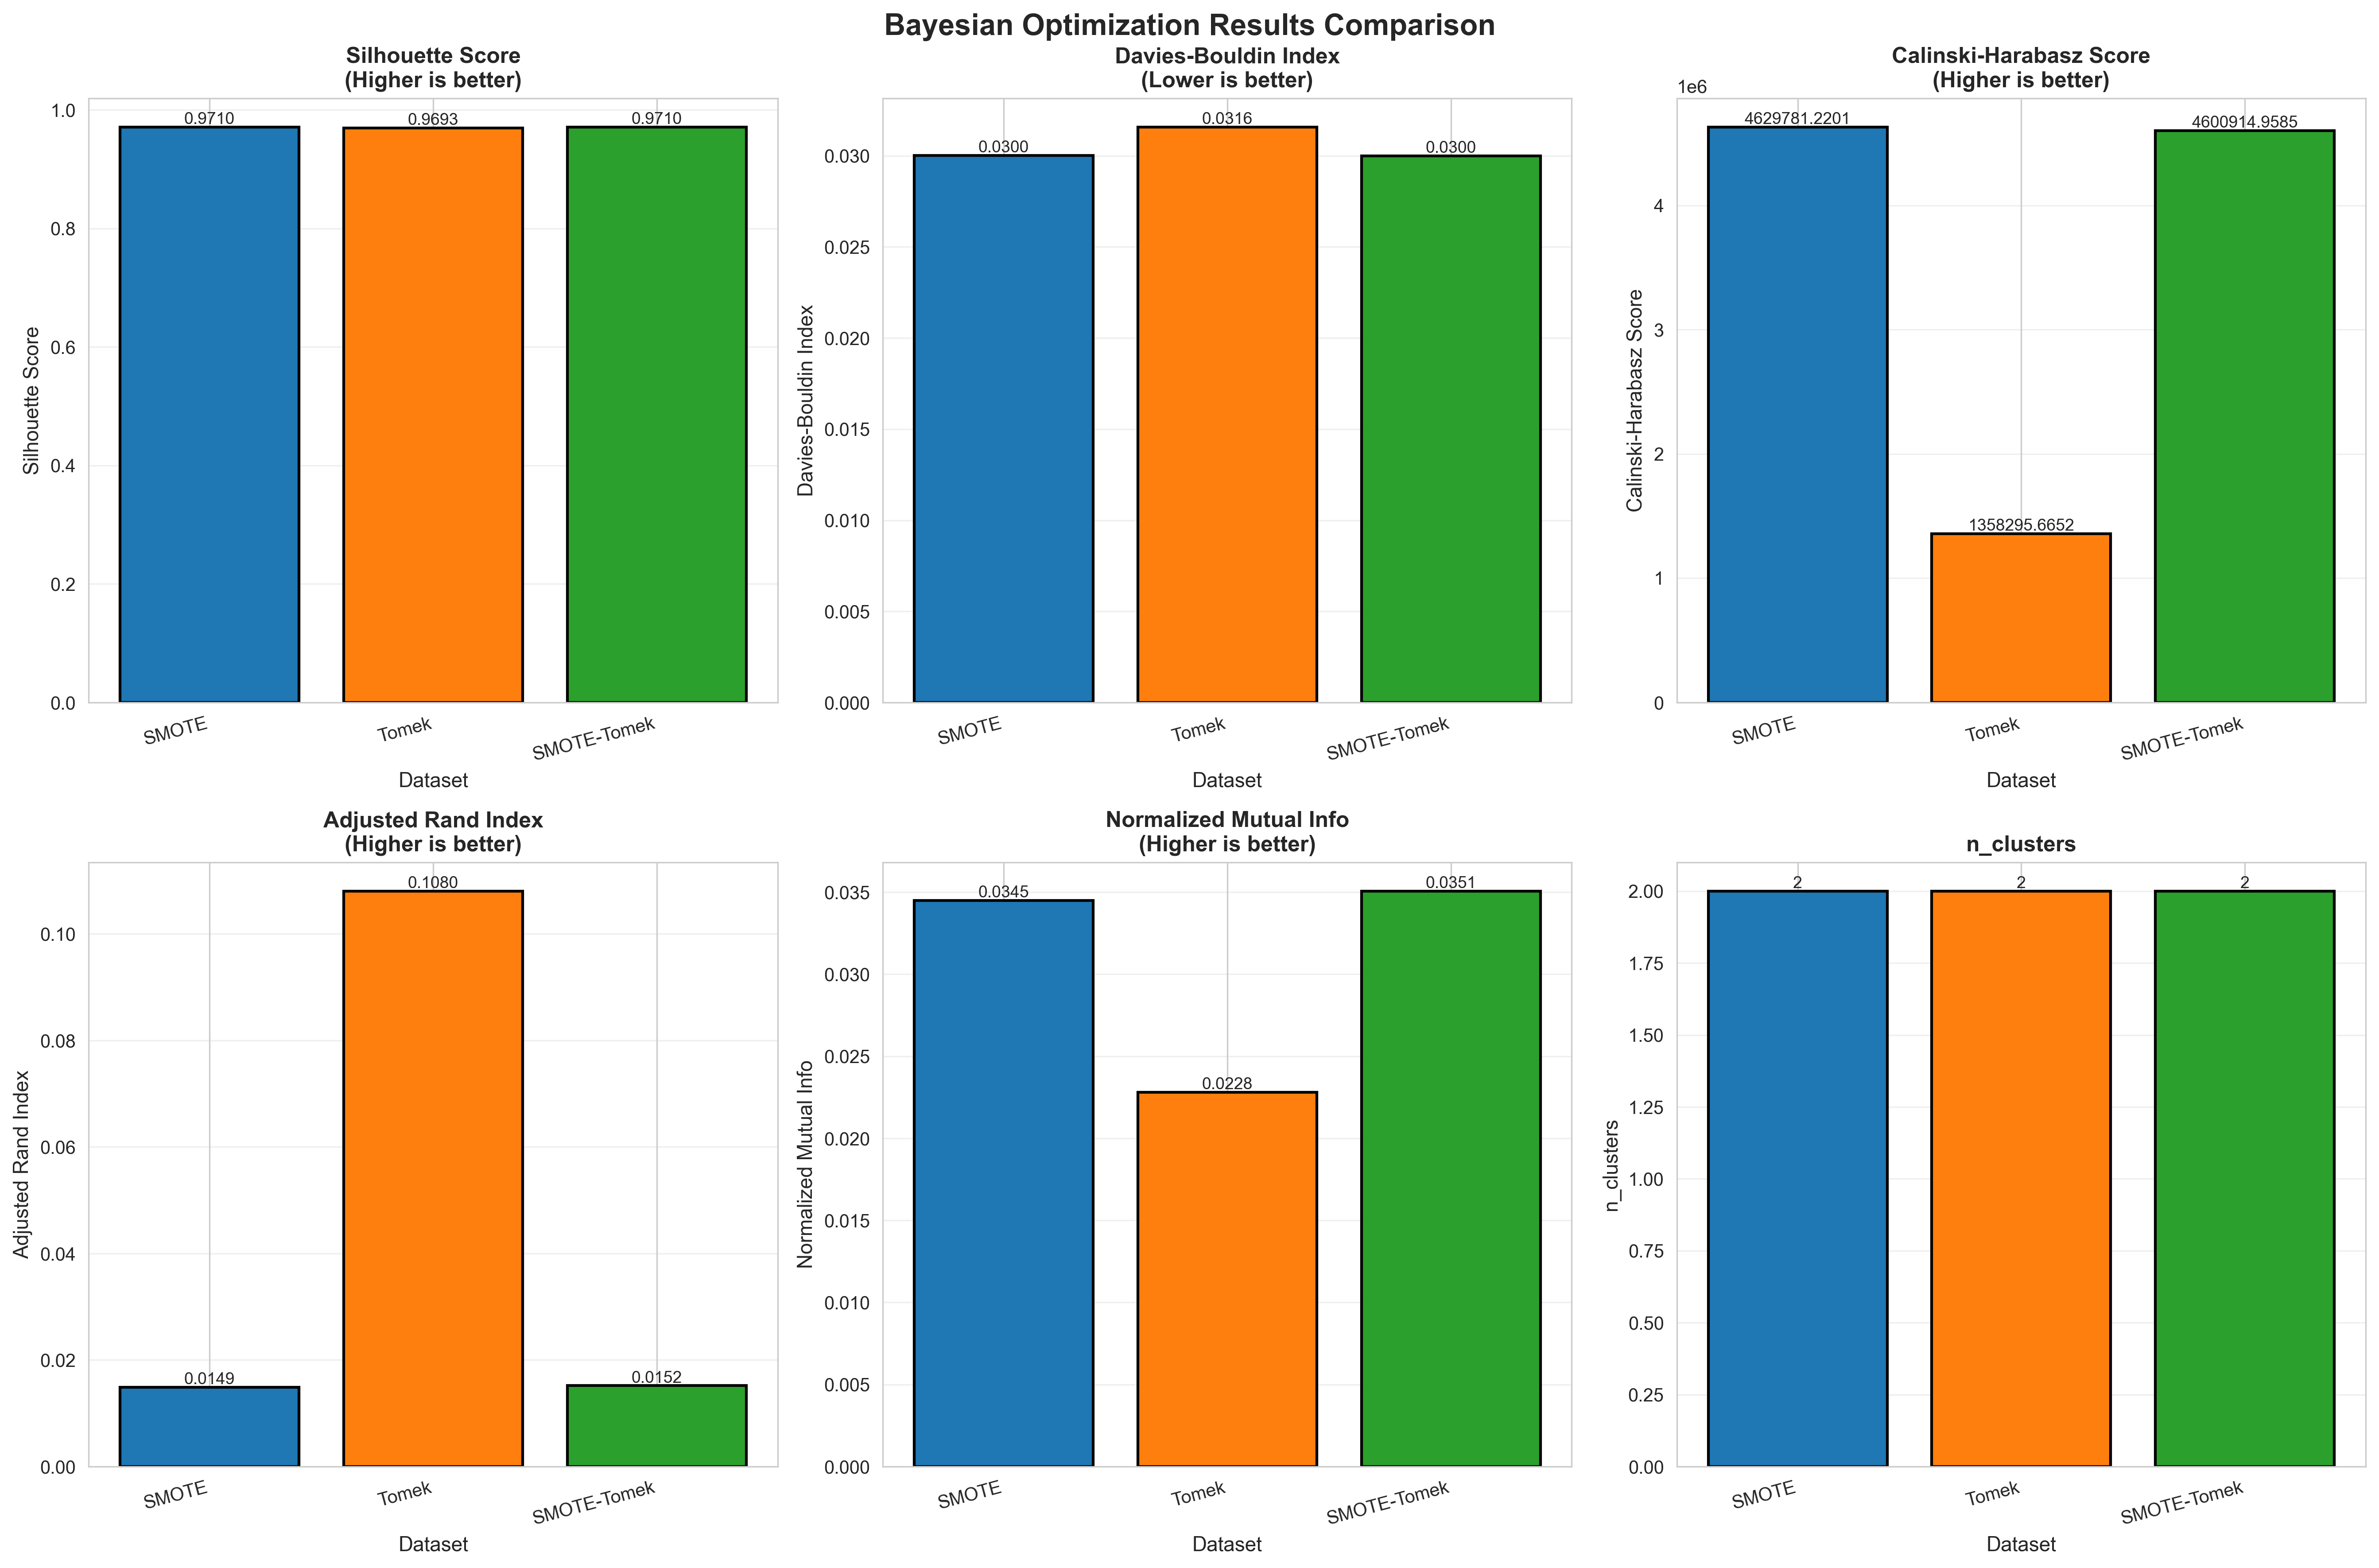
\includegraphics[width=0.6\textwidth]{images/Clarans/bayesopt/bayesian_comparison_all_datasets.png}
\caption{Performance Comparison of Bayesian Optimization Across Resampling Methods.}
\end{figure}


\subsection{From-Scratch Implementation of CLARANS}

\begin{figure}[H]
\centering
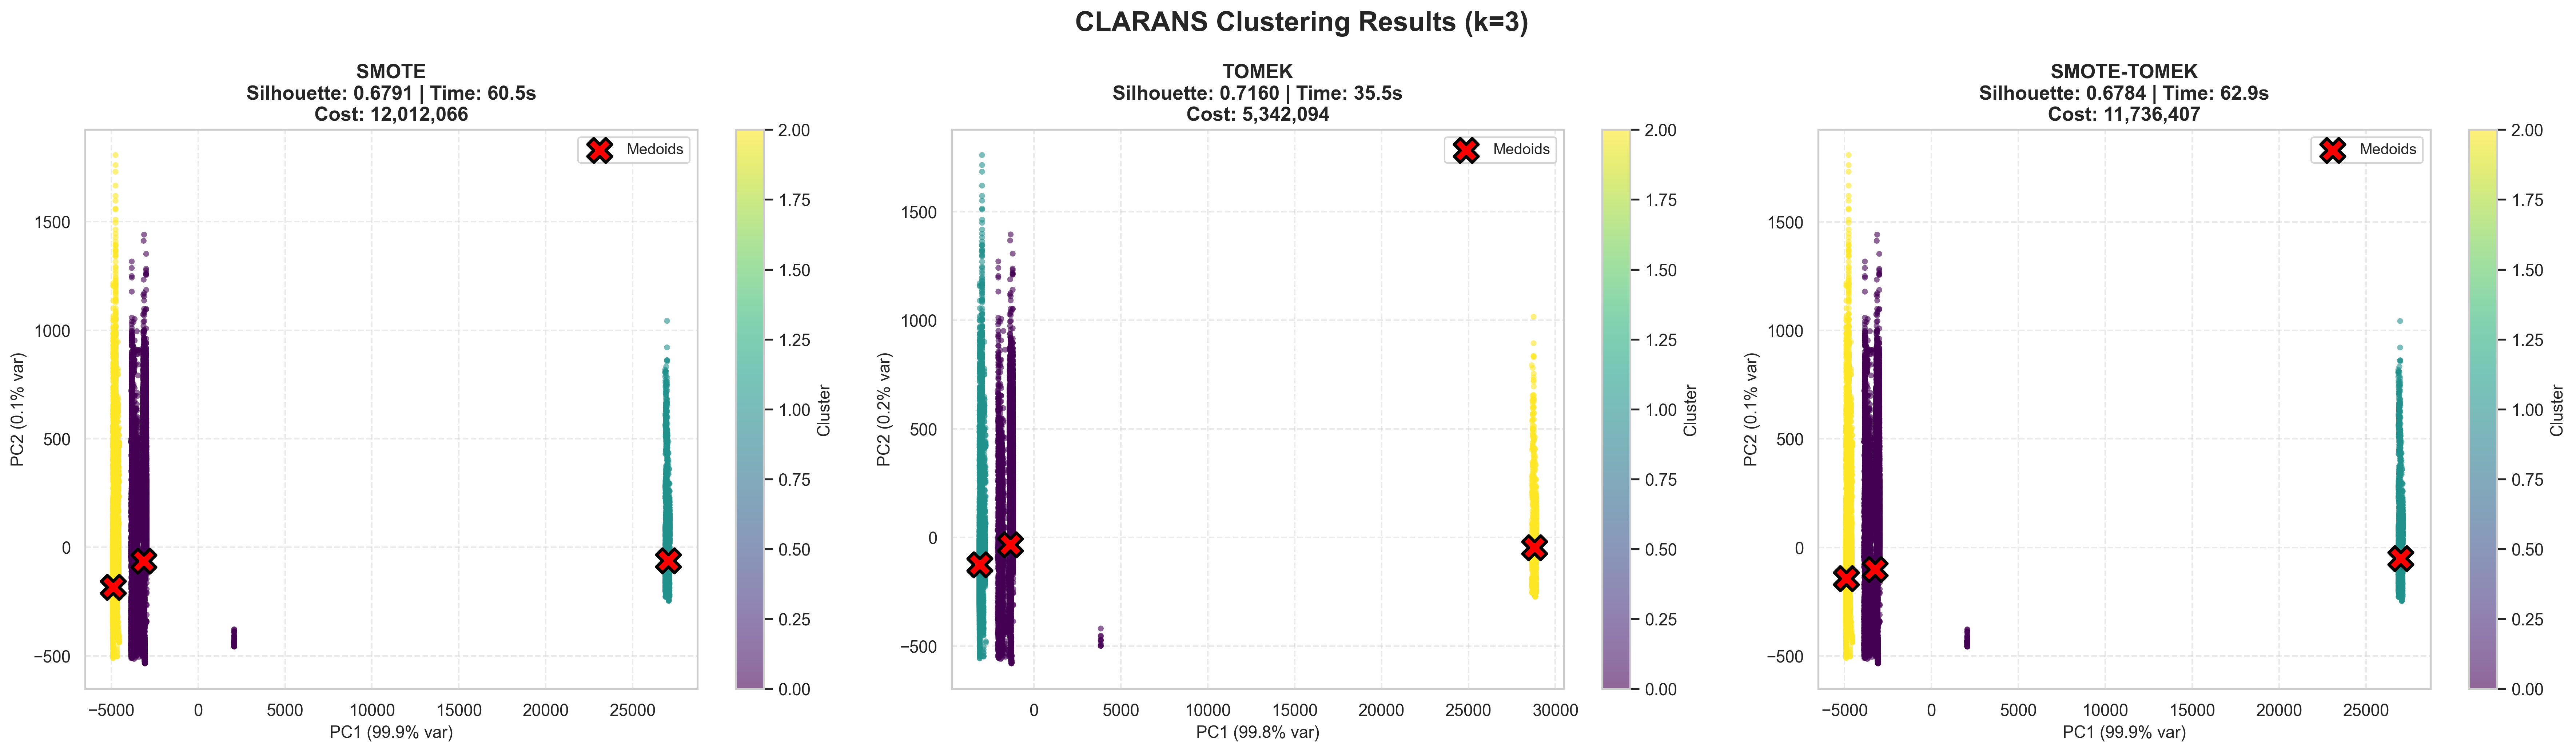
\includegraphics[width=\textwidth]{images/Clarans/scratch/clarans_clustering_results.png}
\caption{2D PCA Projection of CLARANS Clustering Results ($k=3$) on All Three Datasets. Each subplot shows predicted clusters (color-coded), medoids (red crosses), and cluster boundaries. The Tomek dataset (center) exhibits the most distinct cluster separation, as reflected in its superior Silhouette Score.}
\label{fig:clarans_scratch_pca}
\end{figure}

The PCA visualizations reveal the internal structure discovered by CLARANS. In the Tomek dataset, three clusters are clearly separated with minimal overlap in the 2D projection, consistent with its high Silhouette Score (0.7160). The SMOTE and SMOTE-Tomek datasets show more cluster overlap, particularly in the central region where synthetic samples were generated to balance class distributions. The medoids (marked as red crosses) are strategically positioned at the centers of dense regions, demonstrating CLARANS' effectiveness in identifying representative cluster prototypes. The first two principal components capture approximately 40-50\% of the total variance across all datasets, indicating that while the 2D projections provide useful insights, the full 64-dimensional feature space contains additional structure that contributes to the clustering results.

Notably, the randomized local search strategy required exploring 353-973 neighbor configurations per local run before convergence, with the Tomek dataset requiring the most extensive search (973 neighbors in the final local run). This higher exploration effort likely contributed to finding the superior medoid configuration reflected in its better clustering metrics. The algorithm's ability to escape local minima through multiple independent local searches ($numlocal=3$) proved effective, with 2 out of 3 runs yielding cost improvements across the datasets.

Overall, the from-scratch CLARANS implementation successfully validated the algorithm's ability to discover meaningful cluster structures in high-dimensional fire detection data. The results demonstrate that data preprocessing strategy (SMOTE vs. Tomek vs. combined) significantly impacts clustering quality, with boundary-cleaning approaches (Tomek) producing more separable clusters than synthetic oversampling methods.